\documentclass{easychair}

\usepackage{booktabs}
\usepackage{amsmath}
\usepackage[numbers,sort&compress]{natbib}
\usepackage{adjustbox}
\usepackage{etoolbox}

% The AAMAS sources use acmart's \Description for figure alt text.
\newcommand{\Description}[1]{}
\newcommand{\TODO}[1]{\textcolor{red}{\textbf{[TODO: #1]}}}
\newcommand{\Pone}{\textsf{P1a}}
\newcommand{\PER}{\textsc{PER}}
% The supplementary appendices note each table's columns below it.
\newcommand{\tabnote}[1]{\par\vspace{3pt}\begin{minipage}{\linewidth}\footnotesize\setlength{\parindent}{0pt}#1\par\end{minipage}}

\title{Beyond Division of Labor: How Roles Shape Feedback and Recovery in
Multi-Agent Systems}

\author{Anonymous Author(s)}
\institute{Anonymous Institution}

\authorrunning{Anonymous}
\titlerunning{Beyond Division of Labor}

\begin{document}

\maketitle

\begin{abstract}
Multi-agent large language model (LLM) systems routinely rely on
role-playing to divide complex tasks. However, it remains unclear whether
these assigned roles genuinely enforce a division of labor or inadvertently
alter other critical system dynamics. We investigate what roles change
beyond task allocation. By ablating role instructions for three open-weight
models on two reasoning benchmarks (Omni-MATH and SciBench), we isolate the
effect of roles while holding the agents, topology, call budget, and
ground-truth evaluator fixed. Deleting role instructions largely dismantles
functional specialization, yet first-pass accuracy does not degrade.
Instead, roles matter through the decision rights they allocate. A
role-structured Reviewer acts as a strict gatekeeper that often withholds
submissions, so the team receives less external corrective feedback. In
exploratory comparisons where both teams have equal access to feedback,
role-free teams recover from initial failures more often and
achieve higher final accuracy in every setting. The gap vanishes in a post
hoc comparison at equal numbers of evaluator verdicts. In a single exploratory run,
forcing the role-structured team to submit in every cycle raises its
recovery to the role-free level for gemma-4, suggesting that the gap stems
mainly from how often each team submits. We conclude that roles govern information flow and decision
rights as well as work allocation. Consequently, designing and evaluating
effective multi-agent organizations requires looking beyond task division
to explicitly manage feedback loops and decision policies.

\end{abstract}

\section{Introduction}
\label{sec:intro}

Multi-agent systems powered by large language models (LLMs) are commonly
designed around explicit organizational structures and role
assignments~\cite{hong2024metagpt,qian2024chatdev,wu2024autogen}. While
formal diagrams suggest a clear division of labor among components such as
Planners, Executors and Reviewers, the actual execution can diverge from
these intentions~\cite{cemri2025why}. Because the roles are instantiated
only through natural language prompts, agents can ignore their constraints,
leading to a functional collapse in which every agent solves the whole
problem. An accuracy score cannot distinguish such a team from one that
works exactly as drawn. This disconnect raises a fundamental question: what
do assigned roles actually change in practice?

In our experiments, roles do produce the division of labor they prescribe,
yet it buys no better first answer. If specialization is not where roles
pay off, their effect must lie elsewhere. We argue that roles also allocate
decision rights and thereby shape the flow of external information. In a
Planner-Executor-Reviewer (\PER{}) team, the Reviewer acts as a gatekeeper:
by approving a candidate or demanding further deliberation, it decides when
the team consults an external evaluator. This decision is crucial because
the evaluator returns a verdict (PASS or FAIL) and,
after a FAIL, a repair hint, corrective information that internal
deliberation cannot generate. A cautious Reviewer saves evaluations, but under a capped budget
every withheld submission is a missed opportunity to recover from an
error.

To isolate these effects, we hold the actor model (the language model that
plays all three agents), the agent topology, the agent-call budget and the
ground-truth evaluator constant, and vary the organization in two
directions: we ablate every role instruction, and we enforce the division
of labor through typed message formats. Because feedback reaches each agent
through its prompt, a role ablation also rewrites the feedback channel, so
we document the information each condition receives (\S\ref{sec:method}).
In our main comparison both teams have equal access to the evaluator's
verdict and hint, but the realized number and content of verdicts differ,
and this difference is what roles control. Our findings are as follows.
First, roles induce functional specialization, but it does not improve
first-pass accuracy, consistent with prior role
ablations~\cite{dylan2026equal,orogat2026architectural}. Second, roles
create a gatekeeping effect. A role-structured Reviewer often withholds
approval, frequently before any feedback exists, so its team submits less
and receives fewer corrective verdicts; in an exploratory comparison with
equal access to feedback, role-free teams recover from a failed first answer
more often in all five model and benchmark settings and reach higher final
accuracy. Third, the gap stems mainly from feedback opportunities rather
than from how well each team uses feedback: it vanishes in a post hoc
comparison at equal numbers of verdicts, and, in a single exploratory run, forcing the
role-structured team to submit in every cycle (one pass of the three
agents) raises its recovery to the role-free level for the gemma-4 model. Fourth, two methodological
cautions follow: a role ablation that silently removes the feedback channel
can make roles look necessary for repair, and enforcing roles through typed
interfaces loosens the gate but leaves $8\%$ to $17\%$ of enforced trajectories unfinished, so accuracy does not rise. Finally, evaluating multi-agent
organizations requires reporting recovery after a failed first attempt and
treating decision rights and information pathways as part of the
organization's specification (\S\ref{sec:discussion}).

\section{Related Work}
\label{sec:related}

Classical organization-centered multi-agent systems define roles
independently of their occupants, through formal specifications such as
Moise$^+$ and OperA and through norms that institutions regiment or
sanction~\cite{hubner2002moise,dignum2004opera,esteva2001formal,grossi2007ubilex}.
An LLM role prompt, in contrast, is a degenerate case: it states such
constraints in prose but has no mechanism to enforce them. Prompted roles
are accordingly known to be unreliable~\cite{cemri2025why,orogat2026architectural}.
Moreover, an evolved Planner, Executor and Critic team is no better than an
evolved single agent when the number of model calls is held
fixed~\cite{dylan2026equal}, and many reported multi-agent efficiency gains
arise where one agent suffices~\cite{zhang2026rethinking}.

Iterative refinement, tool feedback and multi-agent debate are standard
paradigms~\cite{madaan2023selfrefine,gou2024critic,du2024debate}, yet models
often repeat earlier outputs even under exact verifier
feedback~\cite{jiang2026exactfeedback}, and self-correction degrades
accuracy when the model judges its own answer~\cite{huang2024selfcorrect}.
It does help when an oracle's correct label
serves as a stopping rule~\cite{huang2024selfcorrect}, and our loop is
gated by exactly such an oracle, an evaluator that knows the correct
answer, where more attempts solve more problems~\cite{brown2024monkeys}. The closest study separates reviewer
precision from critique uptake~\cite{yang2026precise} but neither
manipulates the role structure nor equalizes feedback access across
conditions; we do both (Appendix~\ref{app:related}).

\section{Definitions and Measurement}
\label{sec:framework}

\paragraph{Load-bearing components.} A multi-agent organization is defined
by its agents, interaction order, message-passing graph, context-visibility
policy and role contracts. Prohibitive (\textsc{must not}) clauses, such as
instructing the Planner not to state a final answer, are what establish a
division of labor. Because these clauses are only natural-language prompts,
the realized organization need not match the specification. We call a
component \textbf{load-bearing} if removing or altering it reproducibly
degrades task performance under matched call and information budgets, and we apply it separately to first answers and to repairs
(Appendix~\ref{app:loadbearing}).

\paragraph{Functional collapse.} The first deliberation cycle
\emph{collapses} if all three agents independently assert their own final
answers. The pipeline then operates as three sequential solvers rather than
as a division of labor. This is our main measure of functional
specialization. It does not apply to the structurally enforced condition,
whose schema has no answer field. Appendix~\ref{app:measures} defines the
secondary measures.

\paragraph{First pass and recovery.} A \emph{trajectory} is a team's run on
one problem. \emph{First-pass accuracy} grades the first answer the team
submits to the evaluator. It need not come in the first cycle: a
role-structured team may first deliberate internally, without external
feedback. A trajectory that never
submits is graded once on its final answer when the budget runs out, and
that grade is its first pass. Trajectories whose first graded answer is
wrong are \emph{first-pass wrong} (failed, for short), and \emph{recovery} is the share of them
that finish correct. Because recovery conditions on a post-treatment
variable (whether the first answer failed, which the intervention can
change), recovery contrasts are descriptive~\cite{montgomery2018conditioning}.
Final accuracy is reported over all problems.

% Workshop version: the validation paragraph moved to Appendix B.

\section{Intervention}
\label{sec:method}

To ensure a fair comparison, all conditions share the same three agents,
interaction order (Planner, then Executor, then Reviewer), message-passing
graph, agent-call budget and ground-truth evaluator, and, outside
enforcement, the same context visibility. All use greedy decoding at temperature $0$ and stop a trajectory at its
first PASS. How often a team calls the evaluator, by contrast, is an outcome of its
organization (\S\ref{subsec:mechanism}). Apart from the role instructions
themselves, the conditions differ in two respects. First, the repair hint
that follows a FAIL, written with the gold answer in view and instructed
not to reveal it, reaches the role-structured and enforced teams through
each role's advice slot, the template field reserved for feedback, and the
role-free team as an entry in its shared history
(Figure~\ref{fig:pipeline}). Second, the role-free prompt's closing instruction, its footer, asks
every agent for an answer.

\begin{figure}[t]
\centering
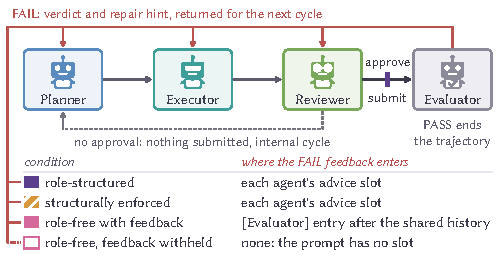
\includegraphics[width=0.585\textwidth]{figures/fig_pipeline.pdf}
\caption{\textbf{One deliberation cycle and where the feedback enters.}
A trajectory (one problem's run, at most six cycles) advances one cycle per
pass of Planner, Executor and Reviewer. The third agent's approval (the bar)
is the only route to the evaluator, which knows the reference answer and
returns a verdict: PASS, ending
the trajectory, or FAIL with a repair hint; without approval the team
deliberates internally in the next cycle. A trajectory that never submits
is graded once (one verdict) when the budget runs out.}
\label{fig:pipeline}
\end{figure}

\paragraph{Role-structured \PER{} (baseline).} Role prompts are as ordinarily written. The Reviewer is instructed to approve only a
complete answer of the expected form and, in a cycle that receives a FAIL,
to route the work back to the Planner or Executor instead of approving.

\paragraph{Role-free with feedback (main comparison).} Every clause that
assigns a function is removed, including the Planner's \textsc{must not}s
and the Reviewer's two clauses on approval. All three agents receive one
identical prompt, ``You are one of three agents collaboratively solving
this problem. Continue the work.'', followed by the problem, the shared history and
the agent's position. The footer asks for its current best answer and a decision to
submit or to keep deliberating. Outside structural enforcement, the third agent's decision to submit is
the team's approval. After a FAIL, all three agents see the verdict and hint as a
shared entry for one cycle, so the two teams have equal access to external
feedback; how many verdicts each draws depends on its submissions.

\paragraph{Role-free, feedback withheld (diagnostic).} The role-free prompt
minus the evaluator's entry shows what a role ablation measures when it
also removes the feedback channel.

\paragraph{Structurally enforced.} Here the interface, not the prompt
wording, enforces specialization. The Planner outputs JSON against a schema
without an answer field, so a final answer is unrepresentable. The Executor receives only the parsed plan, not the
Planner's text, and the Reviewer's acceptance promotes the
Executor's answer by reference. A trajectory terminates when malformed
outputs exhaust the allowed regenerations (Appendix~\ref{app:details}).

\subsection{Pre-registered and exploratory analyses}
\label{subsec:prereg}

We fixed all five pre-specified endpoints (P1 to P5) in writing before
collecting any intervention data. Every test is paired at the problem
level: significance is the exact McNemar test~\cite{mcnemar1947note} on
discordant pairs (problems that exactly one condition gets right), and
bootstrap intervals resample whole problems~\cite{efron1979bootstrap}.
Trajectories that never produce a graded answer count as incorrect, except
in the first-pass contrast. The pre-registered primary endpoint, P4, which
asks whether enforcement's effect on accuracy varies by actor, is null after Holm's correction~\cite{holm1979simple}. We added the role-free condition with feedback, and with it the
main comparison, after the freeze, when the dataset and analysis plan were
fixed. Its design and primary analysis were committed in writing before
any of its data existed, but we classify its results, like those of the
forced-submission run, as exploratory. Appendix~\ref{sec:prereg} details
all endpoints.

\subsection{Experimental setup}
\label{sec:experiments}

We evaluate on the Omni-MATH benchmark of competition
mathematics~\cite{gao2025omnimath}, using $1{,}600$ problems that a seeded manifest
samples uniformly at random from the $4{,}181$ available.
Every condition runs the same problems, so every comparison is paired.
Three actor models are served from one pinned vLLM
server~\cite{kwon2023vllm}: gpt-oss-120b~\cite{openai2025gptoss},
gemma-4-31B~\cite{gemma2026gemma4} and
Llama-3.3-70B~\cite{grattafiori2024llama3}. The pre-registered analysis uses a frozen snapshot of $11{,}600$ Omni-MATH trajectories, including a
context-restored enforcement control (Appendix~\ref{app:details}). In it, the three frozen conditions
(role-structured, feedback withheld and enforced) each run $1{,}600$ problems for gemma-4 and gpt-oss and $400$ for Llama-3.3, and the control runs $400$ for
gemma-4 and for gpt-oss. The evaluator is gpt-oss-120b throughout. After the freeze, we ran the role-free condition with feedback
($4{,}748$ trajectories) on the same server, problems, budget and
evaluator, for all three actors on Omni-MATH and for gemma-4 and gpt-oss on
the SciBench benchmark~\cite{wang2024scibench}, whose role-structured and
feedback-withheld cells (a cell is one actor on one benchmark) were frozen separately. Because decoding at
temperature $0$ is not fully deterministic on a shared server, we treat
each cell as a single sample (Appendix~\ref{app:details}). A single-agent comparison from a separate, earlier corpus is in
Appendix~\ref{app:details}. Prompts, runners, analysis scripts and data manifests will be released.

\section{Results}
\label{sec:results}

% ==========================================================================
% Table 1 (AIAS 2026 workshop copy; caption shortened by
% analysis/scripts/mk_table_collapse_ws.py) -- functional collapse per actor, compact form
%
% GENERATED FILE -- do not edit by hand. Any edit is overwritten.
% generating script : analysis/scripts/mk_tables.py
% canonical input   : analysis/out/FINAL_TABLES_OUTPUT.txt  sections T1, T23
%                    analysis/out/FIGDATA_BF.json  (role-free with feedback: collapse only)
% frozen data       : experiments/results/FROZEN/, frozen_at 2026-09-30T10:09:30.201557
%                     11600 trajectories
%                     sha256 fa22a446d5314bb67b1c6a6444b511eeeae3eb8770419a36f182617eeccbf3b5  actor3.jsonl
%                     sha256 038e08aec4d4aee166106a6325309dfe2301faf339c7d0bf82338a74576424d4  armCp.jsonl
%                     sha256 e4e53cb117d91129991ce2fe87e336e152fc9ee6ca826d363f2bd5dd240d7130  campaign_v2.jsonl
% canonical-output sha256 : b26ccb5451a5eaed14046a27a980ba8797e5669912df907bc25f69bf60ad5b76
% generation date   : 2026-10-04  (derived from the canonical
%                     input's mtime, not wall-clock: regeneration must
%                     be byte-identical)
%
% Compact form of the supplement's full collapse table
% (supp_role_collapse.tex): byte duplication, the enforced row and the
% marker sensitivity live there, built from the same parsed inputs.
% The adjudication is outcome-blind but NOT condition-blind: do not
% describe it as blinded (APPROVED_CLAIMS A1 / DEAD list).
%
% Reader-facing condition names per paper/TERMINOLOGY.md; internal arm
% codes are deliberately absent and their absence is asserted at
% generation time.
% ==========================================================================
\begin{table}[t]
\centering
\caption{\textbf{Functional collapse on the Omni-MATH benchmark.} Share of
first cycles (the first pass of the three agents) in which all three assert
their own final answer, per actor; bold: without roles. RS: role-structured; RF$^{-}$ and RF: role-free with the evaluator's
feedback withheld or shown. \emph{Adjudicated no division}: share of a
judged sample of first cycles in which a model judge with a fixed rubric
(outcome-blind, not condition-blind) finds no division of labor.}
\label{tab:collapse}
\small
\begin{tabular}{@{}l ccc cc@{}}
\toprule
 & \multicolumn{3}{c}{functional collapse} & \multicolumn{2}{c}{adjudicated no division} \\
\cmidrule(lr){2-4}\cmidrule(lr){5-6}
actor & RS & RF$^{-}$ & RF & RS & RF$^{-}$ \\
\midrule
gemma-4-31B & $0.000$ & $\mathbf{0.976}$ & $\mathbf{0.974}$ & $0.000$ & $\mathbf{0.857}$ \\
gpt-oss-120b & $0.120$ & $\mathbf{0.846}$ & $\mathbf{0.883}$ & $0.000$ & $\mathbf{1.000}$ \\
Llama-3.3-70B & $0.000$ & $\mathbf{0.872}$ & $\mathbf{0.900}$ & $0.000$ & $\mathbf{1.000}$ \\
\bottomrule
\end{tabular}
\end{table}


\begin{figure}[t]
\centering
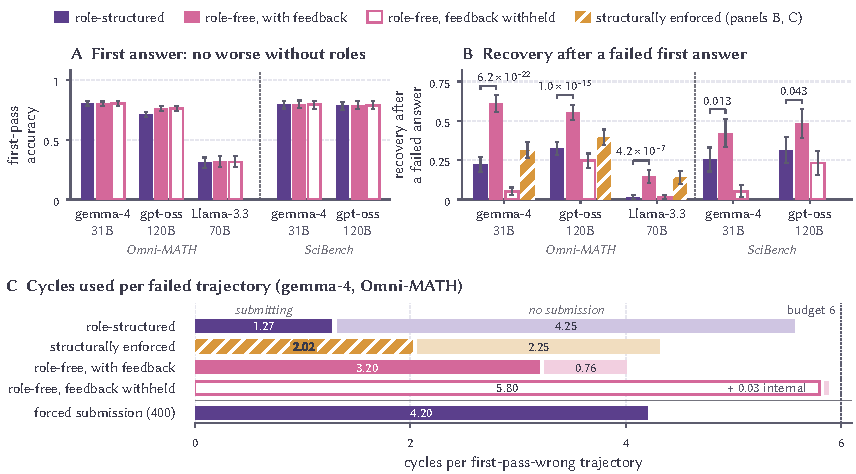
\includegraphics[width=\textwidth]{figures/fig1_v3_story_ws.pdf}
\caption{\textbf{Roles organize the team; the Reviewer's gate limits feedback and recovery.}
\textbf{(A)} First-pass accuracy, over trajectories with a first verdict.
\textbf{(B)} Recovery: the share of first-pass-wrong trajectories (first
graded answer wrong) that finish correct, each condition over its own set; brackets give the exact
McNemar $p$ for role-structured against role-free with feedback, paired on
problems both first answer wrongly. \textbf{(C)} Cycles of gemma-4's first-pass-wrong Omni-MATH
trajectories that end in a submission (the third agent approved) or
internally (it declined); a PASS ends a
trajectory early. Hollow bars: role-free with feedback withheld, a diagnostic. In (B),
enforced trajectories that never finish count as unrecovered.
Bottom row: the
exploratory forced-submission run ($400$ problems). Error bars: bootstrap
$95\%$ intervals.}
\label{fig:dissociation}
\end{figure}

\subsection{R1. Roles create specialization, but not a better first
answer}
\label{subsec:collapse}

Removing role instructions largely eliminates the intended division of
labor for all three actors (gemma-4, gpt-oss and Llama-3.3) on the
Omni-MATH benchmark: functional collapse, the share of first cycles in
which every agent asserts its own final answer, is rare with roles and the
norm without them (Table~\ref{tab:collapse}). The change comes mostly from the Planner; the Executor answers either way. A role-structured
Planner seldom states an answer and a role-free one nearly always does, so the division of labor rests on a single \textsc{must not} clause. Because the role-free footer asks for an answer, the absolute level
partly reflects that request, but the ordering holds under all three
answer-marker definitions, the cues that count as an answer
(Appendix~\ref{sec:collapse_full}). A model judge, outcome-blind but not condition-blind, agrees in direction (Table~\ref{tab:collapse}).

Despite this loss of specialization, first-pass accuracy is largely
unaffected. On problems graded under both conditions, using the frozen feedback-withheld cells, whose inputs equal the role-free team's with feedback
until the first verdict, it is unchanged for gemma-4 and Llama-3.3 and
higher without roles for gpt-oss (Figure~\ref{fig:dissociation}A;
Table~\ref{tab:recovery}). Because one model plays every agent, a Planner
that solves the whole problem brings no competence the Executor lacks;
gpt-oss may gain from extra independent solutions
(Appendix~\ref{app:results}).

\subsection{R2. With equal feedback access, the role-free team recovers more}
\label{subsec:recovery}

%% GENERATED by analysis/scripts/mk_table_main.py --workshop from
%% FIGDATA_BF.json and FIGDATA_GATE.json -- do not edit by hand.
\begin{table}[t]
\centering
\caption{\textbf{Role-structured against role-free with feedback, in every cell} (one actor
on one benchmark; $n$ problems). RS: role-structured; RF: role-free with
the evaluator's feedback shown; RF$^{-}$: role-free with it withheld, a
diagnostic. A trajectory is first-pass wrong when its first graded answer is wrong: its
first submission, or the single end-of-budget grading if it never submits.
\emph{Recovery}: share of first-pass-wrong trajectories that finish
correct, each over its own set. \emph{Recovered only by}: on the $n$
problems both first answer wrongly, those recovered by one condition only,
with the exact McNemar $p$. \emph{Verdict-matched} (post hoc): the same,
with each RF trajectory cut off after as many verdicts as RS received.
\emph{Final accuracy}: over all problems, paired. \emph{Submissions}:
third-agent approvals per first-pass-wrong trajectory. \emph{RS never
submits}: RS first-pass-wrong trajectories with no submission in six
cycles.}
\label{tab:main}
\footnotesize
\setlength{\tabcolsep}{5pt}
\begin{tabular}{@{}l ccc cccc@{}}
\toprule
 & \multicolumn{3}{c}{recovery} & \multicolumn{4}{c}{recovered only by (paired)} \\
\cmidrule(lr){2-4}\cmidrule(lr){5-8}
actor, domain ($n$) & RS & RF & RF$^{-}$ & $n$ & RS & RF & $p$ \\
\midrule
gemma-4, Omni-MATH ($1{,}600$) & $0.222$ & $0.609$ & $0.051$ & $236$ & $4$ & $89$ & $6.2{\times}10^{-22}$ \\
gpt-oss, Omni-MATH ($1{,}600$) & $0.324$ & $0.552$ & $0.247$ & $319$ & $17$ & $101$ & $1.0{\times}10^{-15}$ \\
Llama-3.3, Omni-MATH ($400$) & $0.014$ & $0.147$ & $0.015$ & $250$ & $1$ & $26$ & $4.2{\times}10^{-7}$ \\
\addlinespace
gemma-4, SciBench ($574$) & $0.254$ & $0.419$ & $0.051$ & $100$ & $7$ & $21$ & $0.013$ \\
gpt-oss, SciBench ($574$) & $0.315$ & $0.483$ & $0.231$ & $93$ & $7$ & $18$ & $0.043$ \\
\bottomrule
\end{tabular}

\medskip
\begin{tabular}{@{}l ccc ccc cc c@{}}
\toprule
 & \multicolumn{3}{c}{verdict-matched} & \multicolumn{3}{c}{final accuracy}
 & \multicolumn{2}{c}{submissions} & RS never \\
\cmidrule(lr){2-4}\cmidrule(lr){5-7}\cmidrule(lr){8-9}
actor, domain ($n$) & RS & RF & $p$ & RS & RF & $p$ & RS & RF & submits \\
\midrule
gemma-4, Omni-MATH ($1{,}600$) & $0.165$ & $0.153$ & $0.69$ & $0.846$ & $0.921$ & $1.7{\times}10^{-24}$ & $1.27$ & $3.20$ & $84/316$ \\
gpt-oss, Omni-MATH ($1{,}600$) & $0.229$ & $0.216$ & $0.72$ & $0.803$ & $0.894$ & $2.7{\times}10^{-28}$ & $2.10$ & $3.53$ & $51/463$ \\
Llama-3.3, Omni-MATH ($400$) & $0.012$ & $0.008$ & $1.0$ & $0.315$ & $0.415$ & $1.6{\times}10^{-7}$ & $0.32$ & $2.71$ & $205/276$ \\
\addlinespace
gemma-4, SciBench ($574$) & $0.230$ & $0.190$ & $0.48$ & $0.847$ & $0.880$ & $0.0054$ & $1.95$ & $3.62$ & $3/118$ \\
gpt-oss, SciBench ($574$) & $0.215$ & $0.247$ & $0.68$ & $0.852$ & $0.892$ & $1.9{\times}10^{-4}$ & $2.68$ & $3.95$ & $1/124$ \\
\bottomrule
\end{tabular}
\end{table}


The two teams diverge after a rejected first answer. In this main
comparison, exploratory because it was added after the freeze
(\S\ref{subsec:prereg}), the role-free team recovers more in all five cells (Table~\ref{tab:main}), both over its own failed
trajectories and, paired, on the problems both teams first answer wrongly.
For the gemma-4 model on Omni-MATH, it recovers $0.609$ of its failed
trajectories against $0.222$ (Figure~\ref{fig:dissociation}B).

For gemma-4, both teams reach the same first-pass accuracy and, because a
PASS ends the trajectory, keep every correct first answer, so the extra recoveries carry straight into final accuracy.
In every cell, final accuracy is higher without roles. The recoveries are revisions: nearly every passing
answer differs from the one first rejected (Appendix~\ref{sec:recovery}).
Hints contain the gold answer verbatim in at most $2.3\%$ of failing
verdicts in any cell; we did not audit partial leakage. A second run of the
two gemma-4 cells with feedback is close to the first, though the SciBench
paired test weakens to $p=0.052$ (Appendix~\ref{app:results}). R3 asks
whether the gap reflects how well each team uses a verdict or how many
verdicts it draws.

\subsection{R3. The Reviewer's approval governs feedback opportunities}
\label{subsec:mechanism}

Every submission returns a verdict and, on a FAIL, a repair hint, so each
one is another chance to revise; the two teams differ in how often they
take it. For the gemma-4 model on the Omni-MATH benchmark, the
role-structured team submits $1.27$ times per failed trajectory against
$3.20$ for the role-free team (Figure~\ref{fig:dissociation}C), and it submits less often in every cell. Much of this
withholding happens before any feedback exists, and some failed trajectories never submit, so they never see external feedback
(Table~\ref{tab:main}). On
Omni-MATH, the prompt clause that forbids approval after a FAIL
covers only a minority of the declines for every actor, and in the cycles
it does not cover the Reviewer declines more often than the role-free
team's third agent, by far for gemma-4 and Llama-3.3 (Table~\ref{tab:gate}). The gate therefore
reflects the Reviewer's disposition rather than the letter of its prompt,
plausibly because an agent told to critique searches for flaws.

\paragraph{Removing the gate restores recovery.} To test whether the gate
causes the gap, we kept the role-structured prompts unchanged but submitted
the team's answer in every cycle, overriding the Reviewer. We ran this
exploratory test once, for gemma-4 on the $400$ Omni-MATH problems of a
post-freeze re-run of the role-structured condition
(Appendix~\ref{app:details}). Every cycle then becomes a submission
(Figure~\ref{fig:dissociation}C), and recovery rises from
$0.198$ in that re-run to $0.613$, matching the role-free team on the same
problems (Table~\ref{tab:forced}). First-pass accuracy does not move, so the Reviewer's early declines bought no better first answer but cost
chances to repair it.

\paragraph{At equal verdict counts, the gap disappears.} In a post hoc
comparison on the problems both teams first answer wrongly, we cut each
role-free trajectory after as many verdicts as the role-structured team
received. No cell then shows a significant difference
(Table~\ref{tab:main}), and the pooled difference is $+0.009$ $[-0.014,+0.033]$ in favor of roles. The matching is coarse: a
role-free trajectory cut after a single FAIL cannot recover, so wherever
the role-structured team received one verdict the pair ties at zero, as in
most of gemma-4's pairs. On problems with at least two verdicts the difference remains not significant.
Recoding the scoring defect of \S\ref{sec:limitations} gives roles a small
significant margin on all paired problems, and no variant puts the role-free team significantly ahead
(Table~\ref{tab:robust}). A truncation cannot show that the two teams use
each verdict equally well, but together with the forced-submission run it
indicates that the gap stems mainly from how often the team requests
feedback rather than from how well it uses that feedback.

\paragraph{Without feedback, submitting more does not help.} For gemma-4, with the feedback withheld, the role-free team still
submits in almost every cycle
(Figure~\ref{fig:dissociation}C) but repeats its answer, a single distinct answer in $84.5\%$ of its failed trajectories
($20.8\%$ for gpt-oss; Table~\ref{tab:enforcement}), and rarely recovers;
adding the verdict and hint to the otherwise identical prompts lifts its
recovery (Table~\ref{tab:main}). Against this diagnostic alone, roles would appear load-bearing for repair, clearly so only for gemma-4
(Table~\ref{tab:recovery}).

\subsection{R4. Generality and organizational constraints}
\label{subsec:xdomain}

\paragraph{The pattern recurs on a second domain.} On the text-only slice
of the SciBench benchmark (free-response college science problems), where only the domain wording of the prompts changes,
the gemma-4 and gpt-oss models show the same ordering in recovery and final
accuracy (Table~\ref{tab:main}). The recovery contrast is weaker,
consistent with a looser gate: the role-structured team almost always
submits at least once, and the contrast again vanishes at equal verdict
counts.

\paragraph{Enforcement loosens the gate but is brittle.}
\label{subsec:enforce} On Omni-MATH, with roles enforced through typed message formats, the
Planner never asserts a final answer in the first cycle, whereas it nearly
always does without roles. The enforced team also submits more often,
and where the gate was tightest, for the Llama-3.3 model, recovery rises
close to the role-free team's; for gemma-4 and gpt-oss the direction is the
same but not significant (Appendix~\ref{sec:enforcement}). The gain does not
reach end-to-end accuracy, because $8\%$ to $17\%$ of enforced trajectories
exhaust the allowed regenerations on malformed outputs and never finish.
Under the pre-registered rule, which counts them as incorrect, enforcement
lowers accuracy significantly for gemma-4 and leaves it unchanged for the other two; scoring only the trajectories that finish would suggest
gains for every actor, a survivorship bias (Appendix~\ref{app:results}). In
our implementation, enforcement thus trades one obstacle for another: it loosens the gate but adds a new way to fail.

\section{Discussion}
\label{sec:discussion}

\paragraph{Roles allocate decisions alongside work.} First-pass accuracy
does not depend on the division of labor: without roles it is unchanged, or higher for the gpt-oss model. Except with gpt-oss, teams rarely change a failed answer unless told it
failed. After that signal, the role contract adds little revision capacity. At equal verdict counts the teams do not differ significantly under the
pre-specified scoring, and roles hold a slight edge after the scoring recode of \S\ref{sec:limitations}. The role contract mainly decides when the team asks for evaluation. A role-structured Reviewer
withholds approval, so its team draws fewer verdicts, sometimes just
the final grading.

\paragraph{A design trade-off rather than a defect.} A Reviewer that
withholds approval conserves evaluation calls. This conservatism can be valuable when evaluations are costly, noisy or unavailable. With a
ground-truth evaluator and a fixed cycle budget, however, it limits the
team's opportunities for corrective feedback. We measure this side of the
trade-off, not the full balance of cost and performance. Where a cheap and
reliable verifier exists, our results suggest letting the team submit often and gating on the verifier rather than on an internal critic.

\paragraph{Decision rights and information pathways.} Because feedback
reaches the agents through the role templates, an ablation that rewrites
them can silently remove the feedback channel. A role ablation therefore
needs an information audit alongside budget matching. Just as precise
reviewing does not guarantee that a critique is adopted~\cite{yang2026precise},
a clean division of labor does not guarantee recovery from errors. We recommend reporting performance after a failed first attempt
and measuring the realized organization instead of assuming the specified
one. Who may submit and which agents see the feedback belong to the
organization's specification. Lifelong multi-agent systems, which fail
repeatedly, face these choices throughout deployment.

\section{Limitations}
\label{sec:limitations}

\begin{itemize}
\item \textbf{Oracle-assisted recovery.} The recovery loop is gated by an
oracle, so every reported recovery is oracle-assisted rather than
autonomous self-correction. Stopping at the first PASS hides later
revisions that could undo a correct answer, and an evaluator that can be
queried repeatedly favors the team that queries it most.

\item \textbf{Scope and exploratory status.} We test one \PER{}
organization on text-based reasoning tasks, with an evaluator that is
itself one of the models under study. The main comparison and the
forced-submission run are exploratory, added after the freeze. The
forced-submission run is a single run for one actor on one domain, and it
removes the whole gate, not only the clause forbidding approval after a
failure.

\item \textbf{Feedback and cost.} Equal access to feedback does not
equalize the realized number or content of verdicts, and the two teams see
the feedback in different places. We do not show that any submission
policy is cost-optimal (further disclosures in Appendix~\ref{app:details}).

\item \textbf{Scoring and logging defects.} The runner graded the last
\emph{submitted} answer but recorded the last \emph{held} one, the team's
current answer. For gemma-4 on Omni-MATH they disagree on $17\%$ of
role-structured first-pass-wrong trajectories. Recoding them narrows the
recovery gap and moves the verdict-matched difference toward roles
(\S\ref{subsec:mechanism}, Table~\ref{tab:robust}), but the primary
analysis keeps the pre-specified rule. A logging defect hides most of
gpt-oss's role-free reasoning traces from the record, not from the agents,
and does not create the collapse (Appendix~\ref{app:results}).
\end{itemize}

\section{Conclusion}
\label{sec:conclusion}

Deleting multi-agent roles largely eliminates the intended division of
labor for every model we tested on Omni-MATH, without lowering first-pass
accuracy. Besides dividing work, roles allocate decision rights. A
role-structured Reviewer controls when the team submits to the external
evaluator. In exploratory comparisons with equal access to feedback, the
role-free team recovers from a failed first answer more often in every
tested setting. A post hoc comparison at equal numbers of verdicts removes
this advantage, and so does forcing gemma-4's role-structured team to
submit in every cycle. Roles do not just assign responsibilities; they also
govern decisions and information flow, which shape how a team recovers
from failure. Building an effective multi-agent organization therefore goes
beyond assigning roles correctly. It requires designing decision rights and
information pathways that support the desired system behavior.


\bibliographystyle{plainnat}
\bibliography{refs}

\appendix

\section{Extended related work}
\label{app:related}

\paragraph{Roles in organizational models.} Organization-centered
multi-agent systems give roles a formal existence independent of their
occupants. Moise$^+$ separates structural, functional and \emph{deontic}
specifications~\cite{hubner2002moise}. OperA makes role adoption an explicit
social contract~\cite{dignum2004opera}, and electronic institutions specify
norms outside the agents~\cite{esteva2001formal}, to be regimented
(violation made impossible) or sanctioned~\cite{grossi2007ubilex}. An LLM
role prompt is the degenerate case: functional and deontic clauses in prose,
with nothing to make them bind. Our role-free condition keeps the positions,
the communication graph and the turn order, but deletes these clauses.
Conversely, our enforced condition regiments the functional part at the
interface. In this paper, adaptability means revising an answer across
attempts on the same problem, not reorganizing the
team~\cite{horling2004survey}. Teamwork models make repairing a failed joint
plan a team obligation~\cite{tambe1997flexible}, which a prompt can state
but not secure.

\paragraph{Role specialization and role drift.} Prompted roles are known to
be unreliable. Agents disobey the role specification across annotated
traces~\cite{cemri2025why}, and \emph{role drift} has a training-time
account~\cite{cao2026modules}. Role-label conditioning fails to induce the
intended specialization~\cite{orogat2026architectural}, and agents collapse
into highly similar rationales~\cite{patel2026representational}.
Differentiation can even arise \emph{without} assigned
roles~\cite{kandoussi2026whoami}. Recent enforcement-side work makes role
scope part of the system structure rather than advice in the
prompt~\cite{stettler2026progressive,ge2026roles}. While role drift and the
decoupling of role quality from task performance are
known~\cite{cao2026modules,yang2026precise}, we measure them under a
controlled ablation.

\paragraph{Redundancy and parity.} Dylan et al.~\cite{dylan2026equal} hold
total LLM calls fixed and find an evolved Planner, Executor and Critic team
no better than an evolved single agent. Zhang et
al.~\cite{zhang2026rethinking} find that many reported multi-agent
efficiency gains arise where one agent suffices. This objection is why we
compare against a single agent (\S\ref{sec:method}). On the same premise,
Chen et al.~\cite{chen2026agentslimming} prune redundant agents.

\paragraph{Feedback, revision and answer lock-in.} Iterative refinement with
self-generated or tool
feedback~\cite{madaan2023selfrefine,shinn2023reflexion,gou2024critic} and
multi-agent debate~\cite{du2024debate,liang2024divergent} are standard
patterns. Models often repeat earlier outputs under exact verifier
feedback~\cite{jiang2026exactfeedback}. Under self-reflection, this failure
is called Degeneration-of-Thought~\cite{liang2024divergent}, and belief
entrenchment is studied directly~\cite{oh2026entrenchment}. Huang et
al.~\cite{huang2024selfcorrect} report that self-correction degrades
accuracy only in the \emph{intrinsic} setting, where the model judges its
own answer, and improves it when the correct label serves as a stopping
rule~\cite[see also][]{stechly2024selfverification,kamoi2024when}. Our loop
is gated by such an oracle (an evaluator that knows the correct answer),
where more attempts buy more coverage, the share of problems solved by at
least one attempt~\cite{brown2024monkeys}. This is the regime in which the
role-structured team's restraint costs it. Closest to our lever, Chen et
al.~\cite{chen2026relabeling} vary only the \emph{role label} on a
byte-identical erroneous claim and move explicit-correction rates by $23$ to
$93$ percentage points. However, they do so in a single agent without budget
matching.

\paragraph{Coordination versus capability.}
Canedo~\cite{canedo2026architecture} frames structured specification as a
\emph{capability equalizer} whose value falls with model strength.
Theoretical~\cite{yu2026bottleneck} and
complementary~\cite{dochkina2026drop} accounts agree. Our enforced condition
reproduces that direction only under a scoring rule that drops the
trajectories that never finish. Under our pre-registered rule (fixed in
writing before the data existed), it reverses for the gemma-4 model and
vanishes for the other actors (\S\ref{subsec:enforce}).

\paragraph{Prior studies of one trace corpus, and critique uptake.} Three
studies report on one multi-agent trace corpus on the Omni-MATH
benchmark~\cite{jiang2026confidence,yang2026protocol,yang2026precise}. The closest study separates
reviewer \emph{precision} from critique
\emph{uptake}~\cite{yang2026precise}. It finds that a pipeline reviewer
flags real errors more precisely than broadcast-style peer discussion does.
Yet its correct critique far less often changes the next candidate, and
uptake improves when the critique is placed in the solver's working context.
We ask an organizational question these studies leave open: what the role
structure changes beyond the division of labor, including who decides when
the team asks for correction. None of them manipulates the role structure,
checks that the specified division of labor is realized, or matches feedback
access across conditions.
Elsewhere, the failure to revise is almost always measured in a single
agent, leaving no organization to ablate.


\section{Measures, conditions, analyses and campaign}
\label{app:details}

\subsection{What ``load-bearing'' means here}
\label{app:loadbearing}

An organization is specified by a tuple: agents, an interaction order, a
message-passing graph, a context-visibility policy, and a \emph{role
contract} per agent. A contract asserts that an agent performs some function
(\textsc{must} decompose the problem) or that it does not (\textsc{must not}
state a final answer). Clauses of the second kind make the specification a
\emph{division} of labor. Because a clause is prose handed to a language
model, the \emph{realized} organization is not guaranteed to match it.
Nothing records which clauses were honored.

\textbf{Definition.} A component of an organization is \textbf{load-bearing}
if removing or altering it reproducibly degrades task performance
\emph{under matched call and information budgets}.

The budget clause ensures we test organization rather than scale. Removing
roles alongside agents, calls or context confounds the evaluation. We apply
this definition \emph{per phase}, because a team must first produce an
answer and then repair it if it is wrong. The information clause covers
every channel through which a signal reaches an agent. In a prompted system,
feedback arrives through the same templates that carry the roles.
Consequently, a role ablation can change both the roles and the feedback
channel. A contrast is matched only when it changes one of them
(\S\ref{sec:method}). Matched access does not mean matched use: how many
verdicts a team draws depends on how often it submits.

\subsection{Secondary measures}
\label{app:measures}

\paragraph{Exact output duplication (secondary, a lower bound).} This occurs
when two or more role messages are byte-identical, that is, the same raw
completion character for character. It
bounds collapse from below (Appendix~\ref{sec:collapse_full}) and is never used to compare actors.

\paragraph{Answer authorship, and computation.} We measure whether a Planner
authors a final answer. Structural enforcement leaves the Planner no field
in which to write one, so this measure serves as the manipulation check.
Separately, we track whether a Planner abstains from \emph{computing},
scored as containing no evaluated numeric equality (\textbf{\Pone{}}, the
measure of pre-registered endpoint P1; Appendix~\ref{sec:prereg}). Because \Pone{} scores the absence of a pattern, it rewards
short messages. Therefore, it cannot reliably measure a division of labor,
and we use it only as a fidelity check (Appendix~\ref{sec:prereg}).

\paragraph{Validation.} \Pone{} was hand-adjudicated against a definition
frozen \emph{before} the adjudication sheet was opened. It clears a pre-set
agreement threshold of $0.80$ (Appendix~\ref{sec:collapse_full}).

\subsection{Conditions}

\paragraph{Shared settings.} We vary organization in both directions from one baseline: we remove it, and
we enforce it. All conditions share three agents, one interaction order
(Planner~$\rightarrow$~Executor~$\rightarrow$~Reviewer), the message-passing
graph, context visibility (except under enforcement, below) and the total
call budget. They also use the same verifier and prompt, retry budget,
decoding parameters (temperature $0$, that is, greedy decoding, and
identical \texttt{max\_tokens}), stopping rule (a PASS ends the trajectory)
and grading. Every trajectory in the frozen snapshot (the pre-registered dataset,
\S\ref{sec:experiments}) carries the identical
budget record, so no condition gets more agent calls; how often a team
calls the evaluator is an outcome of its organization. Besides the role
clauses themselves, two things differ. After a FAIL, the evaluator returns a repair
hint, written with the gold answer (the reference solution) in view and
instructed not to reveal it. The role-structured and enforced templates show
the hint to all three agents in the next cycle, each through its role's
advice slot, the template field reserved for the evaluator's feedback
(Figure~\ref{fig:pipeline}). The role-free template has no such slot, so
the role-free team receives the feedback as an entry in its shared history,
and a variant that withholds it serves as a diagnostic. The
role-free footer (the closing instruction of the prompt) also asks every
agent for an answer. Among the deleted role clauses are the role-structured
Reviewer's two clauses on approval.

\paragraph{The structurally enforced condition.} The interface, not the wording, enforces
specialization. The Planner emits JSON (a typed output format) against a
schema with \emph{no answer field}, so a final answer is unrepresentable.
The Executor receives the parsed plan object and the problem, never the
Planner's raw text, and emits a derivation and an answer. The Reviewer emits
a verdict, a target span and a critique. Its \texttt{accept} promotes the
Executor's answer verbatim \emph{by reference}, because it has no field in
which to \emph{author} one. Each function stays with one agent under the
same budget, but the Executor sees less context, and a rejected output can
exhaust the regeneration budget (the number of times a malformed output may
be regenerated). A \emph{context-restored control} repeats this condition
with the shared history restored.


\paragraph{Single-agent reference.} A single agent of the same actor under
the same call cap, on the same Omni-MATH problems, guards against
multi-agent gains that merely mimic one capable
agent~\cite{zhang2026rethinking}. It comes from an earlier, separately
collected corpus, and its two actor arms come from separate runs, so only
the direction within an actor can be read. The comparison cuts both ways.
Against its own single agent, the gemma-4 team is less accurate both with
roles (${-}0.0225$, $p=0.0122$) and without them, feedback withheld
(${-}0.0563$, $p=1.22\times10^{-10}$), whereas the gpt-oss team is more accurate without roles
(${+}0.0294$, $p=0.000678$) and not significantly different with them
(${+}0.0131$, $p=0.152$; Table~\ref{tab:singleagent}). A collapsed gpt-oss team is therefore
not functionally one agent, and more agents do not simply help.

\subsection{Instrumentation and pre-registered analyses}

An intervention that never engages cannot explain an outcome, so we measure
engagement. We log every rejected-and-regenerated output with its reason,
count only role-boundary violations in the enforcement rate, and count
answer-bearing calls per condition. One logging gap is disclosed in
Appendix~\ref{app:results}.

All five endpoints (the pre-specified analyses, numbered P1 to P5) were
fixed in writing and committed before any intervention data existed. The full table, with the
outcome for each, is in Appendix~\ref{sec:prereg}. Units are (problem, actor) pairs,
and all conditions run the same problems, so every test is paired, with
bootstrap intervals that resample whole problems~\cite{efron1979bootstrap}.
The pre-registered primary endpoint, P4, asks whether enforcement's effect
on accuracy differs by actor. It is null: no pairwise
difference-in-differences (enforcement's effect in one actor minus its
effect in another) survives Holm's correction for multiple
comparisons~\cite{holm1979simple} (smallest adjusted $p$-value, $p=0.17$).
Before correction, the $95\%$ bootstrap interval for the Llama-3.3 model
against gemma-4, $+0.040$ $[+0.001,+0.080]$, only just excludes zero, while a
bootstrap test on a separate resample gives $p=0.055$: at this margin the two
disagree, and the contrast does not survive the correction. Only the gpt-oss against gemma-4 contrast had adequate
statistical power for an interaction of plausible size.

The \Pone{} manipulation objective also failed. It required enforcement to
drive Planner computation-abstention to ${\approx}1.0$, but the schema
forbids an \emph{answer}, not a computation. It was re-designated to answer
authorship. The role-structured versus feedback-withheld contrast was
pre-registered as a secondary, exploratory replication of a published null,
and splitting it into phases is post hoc. The role-free condition with
feedback, and with it the main comparison, was added after the freeze (when
the dataset and analysis plan were fixed). Its design and primary analysis
were committed in writing before any of its data existed, but its results
are exploratory, as are those of the forced-submission run
(\S\ref{subsec:mechanism}).
Exclusions were fixed in advance, including the rule that decides
\S\ref{subsec:enforce}: \emph{unparseable trajectories count as incorrect
rather than dropped}.

\subsection{Campaign}

\paragraph{Task and problems.} We use the Omni-MATH benchmark of competition
mathematics~\cite{gao2025omnimath}, sampled by a deterministic seeded
manifest (a fixed, reproducible list of problem identifiers) so that every
prefix of the run is a valid random sample. All conditions run the same
problems, so every comparison is paired. A multiple-choice benchmark was
ruled out before launch: on a four-option item, producing a different
candidate succeeds one time in three by chance, which would inflate
recovery.

\paragraph{Actors and scale.} Three actor models are served from one pinned
vLLM server~\cite{kwon2023vllm}: gpt-oss-120b~\cite{openai2025gptoss},
gemma-4-31B~\cite{gemma2026gemma4} and
Llama-3.3-70B~\cite{grattafiori2024llama3}. The pre-registered analysis reads one
frozen snapshot of $11{,}600$ trajectories, $83{,}320$ role messages and
$17{,}486$ gradings on $1{,}600$ problems
sampled uniformly at random from the $4{,}181$ available. The three frozen
conditions run $1{,}600$ problems per cell (one actor on one benchmark) for gemma-4 and gpt-oss and $400$ for Llama-3.3. The
context-restored control covers gemma-4 and gpt-oss at $400$ each. The
evaluator is gpt-oss-120b in every cell, itself one of the actors under
study (\S\ref{sec:limitations}). The single-agent comparator is \emph{not}
part of this campaign; it comes from an earlier, separately collected corpus
on the same benchmark, joined by problem identifier. Power simulated from
that corpus is high for the paired per-actor main effect
(Appendix~\ref{sec:prereg} for the interaction). An early campaign, stopped when
outputs cut off at the token limit were counted as role-boundary rejections,
was never pooled (Appendix~\ref{sec:enforcement}).

\paragraph{The role-free condition with feedback.} It was run after the freeze
($4{,}748$ trajectories) on the same server, problems, budget and evaluator,
for all three actors on Omni-MATH and for gemma-4 and gpt-oss on the
SciBench benchmark~\cite{wang2024scibench}. Its data are manifested
separately and never pooled into a frozen cell. The two gemma-4 cells were
run a second time, independently. A re-run (the first of two; Appendix~\ref{sec:recovery}) of gemma-4's role-structured
condition on $400$ frozen problems shows no detectable drift in final
accuracy ($0.818$ against $0.825$ frozen, paired $p=0.75$), although
recovery moves from $0.146$ frozen to $0.198$. Decoding at temperature $0$ is not deterministic on a
shared server. The two role-free conditions are byte-identical until the
first verdict, yet they agree on gemma-4's first verdict for $1{,}496$ of
$1{,}598$ problems, and their first-cycle collapse differs by up to $0.04$
(Table~\ref{tab:collapse}). We therefore treat a cell as one sample and give
the second run, where we have one, in Appendix~\ref{sec:recovery}. Prompts, runner,
analysis scripts and data manifests will be released with the paper.

\subsection{Further limitations}

\paragraph{Scope, provenance, and experimental disclosures.} We test one
\PER{} organization, with an evaluator that is itself one of the models
under study. While the ordering returns across a second domain of college
science problems, the findings are limited to text-based reasoning tasks.
The role-free condition with feedback, on which the main comparison rests,
and the forced-submission run are exploratory follow-ups, added after the
freeze and outside the pre-registration. The forced-submission
run covers only one actor, one domain, and a single run, and it removes the
entire gate rather than only the clause forbidding approval after a failure.
Matched access to feedback does not match the realized number or content
of verdicts, and we do not show that any submission policy is cost-optimal.
The condition with feedback also differs in feedback presentation:
role-structured agents receive feedback inside role-specific instructions,
whereas role-free agents view it as a bare \texttt{[Evaluator]} entry.
Finally, the context-restored control is only a \emph{partial} control due
to one-sided attrition (Appendix~\ref{sec:enforcement}), and our functional measure
only detects whether every agent asserted an answer, not whether their
reasoning was identical.

\section{Additional results}
\label{app:results}

\paragraph{First-pass accuracy of gpt-oss.} The gpt-oss model may gain
at first pass without roles because its answers vary between derivations
(\S\ref{subsec:mechanism}), so extra independent solutions add chances to be
right; we did not test this.

\paragraph{Content duplication.} For the gemma-4 and
Llama-3.3 models, the role-free Planners write full solutions before boxing
an answer, and their messages share far more numbers with the Executor's
than with roles, so the Executor redoes the Planner's work (Appendix~\ref{sec:collapse_full}). 



\paragraph{A logging defect.} \label{subsec:logging} Our runner recorded
a response's hidden reasoning trace only when its visible content was
empty, so most of gpt-oss-120b's role-free derivations ($75.7\%$ of
messages) are missing from the record (Appendix~\ref{sec:collapse_full}). Agents pass content
only, in every condition, so the defect is in the record alone and leaves
no point estimate of gpt-oss's duplication. It does not manufacture the
collapse: in first cycles with no affected message ($106$ without roles),
role-free collapse is $0.821$ and role-structured $0.118$.



\paragraph{Leakage and reproducibility.} A hint written with the gold
answer in view could hand it over. Hints contain it verbatim in at most
$2.3\%$ of failing verdicts in any cell, and dropping the gemma-4
trajectories on Omni-MATH that saw one barely moves either recovery rate
(Appendix~\ref{sec:recovery}); we did not audit partial leakage. A second, independent run of the two gemma-4 cells with feedback
is close to the first, though the paired test on the SciBench benchmark
weakens from $p=0.013$ to $0.052$; we report the first run throughout
(Appendix~\ref{sec:recovery}).



\paragraph{Structural enforcement.} \label{app:enforce} Enforced and role-structured prompts carry the same advice slot, so this
contrast is matched on feedback access. Enforcement replaces the behavioral
request with a constraint: the Planner's final answer becomes
unrepresentable. The manipulation check passes: the Planner asserts a final
answer in $0.000$ of enforced first cycles for all three actors, against at
least $0.889$ without roles. Enforcement does not change what the Planner
\emph{computes}, so the adjudication still finds no functional division in
$0.071$ to $0.188$ of enforced first cycles: an agent can be structurally
stopped from answering without being stopped from doing the work. It does
loosen the gate: the enforced team submits more often for every actor and,
with more hints arriving, unlocks the answer for gemma-4 and Llama-3.3
(Appendix~\ref{sec:enforcement}).

Recovery rises most where the gate was tightest. Llama-3.3's
role-structured team almost never submits, and under enforcement its
recovery rises about tenfold, from $0.014$ to $0.139$
($p=3.8\times10^{-6}$), close to the role-free team's $0.147$. For gemma-4
and gpt-oss the direction is the same ($p=0.30$ and $0.11$) but not
resolvable against attrition: enforced trajectories that died after an
incorrect first verdict count as unrecovered, as the pre-registration
requires.

Improved revisability does not become end-to-end accuracy, because
enforcement is brittle. A malformed or boundary-violating output must be
regenerated, and when the regeneration budget runs out the trajectory dies:
$8.0\%$, $9.9\%$ and $17.0\%$ of enforced trajectories never finish,
against at most $2.5\%$ in any other condition, and the weakest actor
breaks the schema most often (Appendix~\ref{sec:enforcement}). Under the pre-registered rule,
which counts these trajectories as incorrect, enforcement changes accuracy
by $-0.0225$, $-0.0050$ and $+0.0175$ for gemma-4, gpt-oss and Llama-3.3:
one significant negative and two nulls. Dropping them instead gives gains
for all three actors, all significant and ordered by actor weakness,
matching the direction reported for the capability
equalizer~\cite{canedo2026architecture}. That reading is survivorship bias,
since it scores only the trajectories that finished. Restoring the shared
history at fixed enforcement helps gemma-4, mostly through fewer
trajectories dying, and not gpt-oss (Appendix~\ref{sec:enforcement}).


% The supplementary appendices: the AAMAS supplement's table style and float
% placement, which apply only from here on.
\AtBeginEnvironment{table}{\small\setlength{\tabcolsep}{4pt}}
\AtBeginEnvironment{table*}{\small\setlength{\tabcolsep}{4pt}}
\renewcommand{\topfraction}{0.9}
\renewcommand{\textfraction}{0.07}
\renewcommand{\floatpagefraction}{0.8}
\setcounter{topnumber}{3}
\setcounter{totalnumber}{4}
% GENERATED by scripts/mk_workshop_appendix.py from paper/supplement.tex -- do not edit by hand.
\section*{Detailed results and disclosures}

The main text states every claim it makes and is complete without the
appendices that follow. They give the full numeric backing behind some of
its sentences, in the order of its results: the realized organization (R1,
Appendix~\ref{sec:collapse_full}), recovery (R2,
Appendix~\ref{sec:recovery}), the submission gate (R3,
Appendix~\ref{sec:gate}), and the second domain and structural enforcement
(R4, Appendices~\ref{sec:xdomain} and~\ref{sec:enforcement}), followed by
the pre-registered endpoints (Appendix~\ref{sec:prereg}) and the
single-agent comparator (Appendix~\ref{sec:singleagent}). Every table is generated by a script from the manifested data
(the frozen snapshot, or the separately manifested post-freeze runs) with
the same scripts and outputs as the main text's tables, except the
single-agent comparator, which comes from an earlier, separately collected
corpus. The four figures are generated from the same outputs.

\paragraph{Terms used throughout.} A \emph{trajectory} is one problem's run
through the pipeline, at most six \emph{cycles} of Planner, Executor and
Reviewer. A cycle ends in a \emph{submission} to the evaluator when the
third agent approves the current answer, and in a \emph{decline} otherwise;
each submission returns a \emph{verdict}, PASS or FAIL, and on a FAIL a
repair hint. \emph{First pass} is whether the first submitted answer is
correct; a trajectory that never submits is graded once when its budget
runs out, and that grade is its first pass. \emph{Recovery} is the share of
\emph{first-pass-wrong} trajectories that finish correct. Recovery is
reported on two populations that must not be read across: the
\emph{marginal} population is every first-pass-wrong trajectory of a
condition, on that condition's own denominator; the \emph{paired}
population is only the problems first-pass wrong under both conditions
being compared, on one shared denominator, and it is the population every
test of recovery uses. Tests are exact McNemar tests on the problems that
exactly one condition gets right; intervals are $95\%$ bootstrap intervals
that resample problems; where several tests form a family, $p$ values are
corrected with Holm's step-down procedure. Two \emph{scorings} recur: the
\emph{pre-registered} scoring counts a trajectory that never produced a
graded answer as incorrect, and the \emph{as-graded} scoring drops it. The
conditions are abbreviated RS (role-structured: Planner, Executor and
Reviewer prompts), RF (role-free: one generic prompt for all three agents,
with the evaluator's feedback shown), RF$^{-}$ (role-free with the feedback
withheld) and SE (structurally enforced: the same roles imposed by typed
message formats). The actors are the gemma-4-31B-it, gpt-oss-120b and
Llama-3.3-70B-Instruct models, each playing all three agents.

\section{The realized organization (R1)}
\label{sec:collapse_full}

The main text reports that deleting the role clauses makes every agent
assert its own final answer. Table~\ref{tab:collapse_full} is the full form
of its Table~1, with two further measures and the enforced condition, and
Figure~\ref{fig:roles} shows which agent changes.

% Workshop copy (scripts/mk_workshop_appendix.py): paper/tables/supp_role_collapse.tex with its tabular in an adjustbox; numbers unchanged.
% ==========================================================================
% Supplement -- functional collapse per actor, all three measures
%
% GENERATED FILE -- do not edit by hand. Any edit is overwritten.
% generating script : analysis/scripts/mk_tables.py
% canonical input   : analysis/out/FINAL_TABLES_OUTPUT.txt  sections T1, T18, T20, T23
%                    analysis/out/FIGDATA_BF.json  (role-free with feedback: collapse only)
% frozen data       : experiments/results/FROZEN/, frozen_at 2026-09-30T10:09:30.201557
%                     11600 trajectories
%                     sha256 fa22a446d5314bb67b1c6a6444b511eeeae3eb8770419a36f182617eeccbf3b5  actor3.jsonl
%                     sha256 038e08aec4d4aee166106a6325309dfe2301faf339c7d0bf82338a74576424d4  armCp.jsonl
%                     sha256 e4e53cb117d91129991ce2fe87e336e152fc9ee6ca826d363f2bd5dd240d7130  campaign_v2.jsonl
% canonical-output sha256 : b26ccb5451a5eaed14046a27a980ba8797e5669912df907bc25f69bf60ad5b76
% generation date   : 2026-10-04  (derived from the canonical
%                     input's mtime, not wall-clock: regeneration must
%                     be byte-identical)
%
% Byte duplication is a LOWER BOUND (precision 1.000, recall 0.262)
% and never carries the collapse claim alone (APPROVED_CLAIMS A1).
% The adjudication is outcome-blind but NOT condition-blind: do not
% describe it as blinded (APPROVED_CLAIMS A1 / DEAD list).
%
% Reader-facing condition names per paper/TERMINOLOGY.md; internal arm
% codes are deliberately absent and their absence is asserted at
% generation time.
% ==========================================================================
\begin{table}[t]
\centering
\caption{Functional collapse on the Omni-MATH benchmark under three measures, with the structurally enforced condition and a sensitivity analysis over answer markers.}
\label{tab:collapse_full}
\begin{adjustbox}{max width=\textwidth}\begin{tabular}{@{}lccc@{}}
\toprule
 & functional & exact byte & adjudicated \\
actor & collapse & duplication & no division \\
\midrule
\multicolumn{4}{@{}l}{\emph{role-structured (RS)}} \\
\quad gemma-4-31B-it & $0.000$ & $0.000$ & $0.000$ \\
\quad gpt-oss-120b & $0.120$ & $0.000$ & $0.000$ \\
\quad Llama-3.3-70B-Instruct & $0.000$ & $0.000$ & $0.000$ \\
\addlinespace
\multicolumn{4}{@{}l}{\emph{role-free, feedback withheld (RF$^{-}$)}} \\
\quad gemma-4-31B-it & $\mathbf{0.976}$ & $0.000$ & $\mathbf{0.857}$ \\
\quad gpt-oss-120b & $\mathbf{0.846}$ & $0.680^{\dagger}$ & $\mathbf{1.000}$ \\
\quad Llama-3.3-70B-Instruct & $\mathbf{0.872}$ & $0.008$ & $\mathbf{1.000}$ \\
\addlinespace
\multicolumn{4}{@{}l}{\emph{role-free, with feedback (RF)}} \\
\quad gemma-4-31B-it & $\mathbf{0.974}$ & -- & -- \\
\quad gpt-oss-120b & $\mathbf{0.883}$ & -- & -- \\
\quad Llama-3.3-70B-Instruct & $\mathbf{0.900}$ & -- & -- \\
\addlinespace
\multicolumn{4}{@{}l}{\emph{structurally enforced (SE)}} \\
\quad all actors & n/a & $\leq 0.001$ & $0.071$--$0.188$ \\
\bottomrule
\end{tabular}\end{adjustbox}

\tabnote{RS: role-structured prompts; RF$^{-}$ and RF: role-free prompts with the evaluator's feedback withheld or shown (RF was run after the freeze); SE: structural enforcement. Functional collapse: share of first cycles in which all three agents assert their own final answer. Exact byte duplication: share of first cycles in which two or more of the three messages are identical character for character, a lower bound on collapse that is never used to compare actors. Adjudicated no division: share of a judged sample of first cycles in which a model judge with a fixed rubric finds no division of labor; the judge did not see the grade but could infer the condition. Collapse is not applicable under SE, whose Planner schema has no answer field; for RF only functional collapse was measured. \emph{Sensitivity.} Under three answer-marker definitions the
feedback-withheld role-free rate is $0.846$--$0.999$; the
role-structured rate is $0.000$--$0.238$ under the two stricter
markers and $0.328$--$0.892$ under the loosest, which
also counts any ``therefore'', ``hence'' or ``$=$\,number'' (as when a
Planner restates givens), so read the role-structured level as ``low,'' not
a point estimate. The ordering holds in all 9 of 9
actor$\times$marker cells. $^{\dagger}$Not interpretable: $80\%$ of this cell's planner messages are under $500$ visible characters (the logging defect of Appendix~\ref{app:results}).}
\end{table}


\begin{figure}[t]
\centering
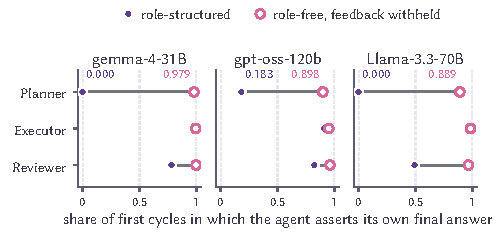
\includegraphics[width=0.585\textwidth]{figures/fig_supp_roles.pdf}
\Description{Three panels, one per actor. Each shows three horizontal
dumbbells, for the Planner, Executor and Reviewer, from the role-structured
value to the role-free value of the share of first cycles in which that
agent asserts its own final answer. The Planner's dumbbell spans almost the
whole axis in every panel; the Executor's is near one at both ends; the
Reviewer's is short.}
\caption{Which agent changes when the role clauses are deleted. For each
actor, the share of first cycles in which the Planner, Executor and
Reviewer assert their own final answer under role-structured prompts
(filled) and under role-free prompts with the evaluator's feedback withheld
(hollow), on the Omni-MATH benchmark. The Planner moves from almost never
answering to almost always answering; the Executor answers under both; the
Reviewer moves less.}
\label{fig:roles}
\end{figure}

\paragraph{The Planner is the agent that changes.} By role, the share of
first cycles in which an agent asserts its own final answer moves from RS
to RF$^{-}$ as follows, for gemma-4-31B-it, gpt-oss-120b and
Llama-3.3-70B-Instruct in turn: Planner $0.000$, $0.183$ and $0.000$ to
$0.979$, $0.898$ and $0.889$; Executor $0.973$, $0.907$ and $1.000$ to
$0.993$, $0.951$ and $0.982$; Reviewer $0.781$, $0.823$ and $0.492$ to
$0.998$, $0.961$ and $0.965$. The Executor's job is to produce the answer,
so it answers under both conditions. The Reviewer often states an answer
even with roles, plausibly because approving an answer tends to restate it.
The division of labor therefore rests on the Planner's single prohibition,
and the role-free footer, which asks every agent for its current answer,
lifts it.

\paragraph{Without roles, Planner and Executor compute the same quantities.} The numbers
in a Planner's first-cycle message and in the Executor's overlap more than
Planner and Executor messages from different problems in the same condition
do, by $+0.449$, $+0.680$ and $+0.432$ without roles against $+0.159$,
$+0.167$ and $+0.145$ with them (Jaccard similarity of the two number
sets). Under roles the Planner writes a plan and the Executor computes;
without them both compute the same quantities. The gpt-oss-120b value
without roles is not interpretable, because most of those Planner messages
are only a few characters long (the logging defect below).

\paragraph{A second opinion from a model judge.} A frontier model rated the
first cycles of $171$ sampled trajectories ($42$ RS, $56$ RF$^{-}$ and the
rest SE) against a rubric frozen before the first judgment, asking whether
a division of labor was realized. Its verdicts agree with the
functional-collapse measure (Table~\ref{tab:collapse_full}), and across the
three rubric questions checked for stability its repeated judgments agree
on $0.947$ to $0.959$ of the items. The judge did not see the grade, but it
could infer the condition, because role words were renamed rather than
equalized across conditions; the collapse claim therefore does not rest on
it.

\paragraph{The logging defect, in detail.} A message whose hidden reasoning
was discarded is short but slow, so we mark messages with fewer than $10$
visible characters per second of latency. They are $75.7\%$ of
gpt-oss-120b's role-free messages and $7.7\%$ of its role-structured ones,
and $93.4\%$ and $22.7\%$ of its first cycles contain at least one. The
runner's own fallback flag marks only $5.8\%$ and $2.7\%$ of the same
messages, so the flag undercounts the defect. For the other two actors
at most $0.5\%$ of messages are marked. The defect cannot have produced the
collapse: on first cycles with no marked message, gpt-oss-120b's functional
collapse is $0.821$ ($n=106$) without roles and $0.118$ ($n=1{,}236$) with
roles.

\paragraph{Validating the computation-abstention measure.} \Pone{}, the
pre-registered measure of whether a Planner abstains from computing, was
checked by hand on $72$ Planner messages against a definition frozen before
the adjudication sheet was opened, each judgment with a recorded reason. It
agrees with the hand labels on $0.903$ of messages (Cohen's $\kappa=0.806$;
precision $0.943$, recall $0.868$), clearing the pre-set $0.80$ threshold.
Agreement fell from $0.967$ at $n=30$ as adjudication continued, and we
report the final figure. Its residual errors point in opposite directions
(symbolic results with no digits are missed, restated givens are flagged),
so they do not push the measure one way.

\section{Recovery (R2)}
\label{sec:recovery}

The main text reports that, with the same access to feedback, the
role-free team recovers more, and that against the feedback-withheld
diagnostic the roles would look load-bearing (the main text's R3).
Table~\ref{tab:recovery} gives that frozen feedback-withheld comparison on
both populations, so the marginal rates and the paired test
can be checked against each other; the comparison with feedback is the main text's Table~2.

% Workshop copy (scripts/mk_workshop_appendix.py): paper/tables/main_recovery.tex with its tabular in an adjustbox; numbers unchanged.
% ==========================================================================
% Table 2 (manuscript) -- first pass and recovery
%
% GENERATED FILE -- do not edit by hand. Any edit is overwritten.
% generating script : analysis/scripts/mk_tables.py
% canonical input   : analysis/out/FINAL_TABLES_OUTPUT.txt  sections T1, T3, T4
% frozen data       : experiments/results/FROZEN/, frozen_at 2026-09-30T10:09:30.201557
%                     11600 trajectories
%                     sha256 fa22a446d5314bb67b1c6a6444b511eeeae3eb8770419a36f182617eeccbf3b5  actor3.jsonl
%                     sha256 038e08aec4d4aee166106a6325309dfe2301faf339c7d0bf82338a74576424d4  armCp.jsonl
%                     sha256 e4e53cb117d91129991ce2fe87e336e152fc9ee6ca826d363f2bd5dd240d7130  campaign_v2.jsonl
% canonical-output sha256 : b26ccb5451a5eaed14046a27a980ba8797e5669912df907bc25f69bf60ad5b76
% generation date   : 2026-10-04  (derived from the canonical
%                     input's mtime, not wall-clock: regeneration must
%                     be byte-identical)
%
% EVERY figure names its population. The marginal and paired
% panels have DIFFERENT denominators and are not interchangeable;
% conflating them has already caused one error in this project.
% Recovery denominator = judged(r) and fp(r)==0: a recorded
% incorrect FIRST verdict, INCLUDING trajectories that later died
% in regeneration (STATISTICAL_AUDIT FATAL-1). Not graded(r).
% Significance is exact McNemar on discordant pairs, never a
% bootstrap CI bound (that label was seed-dependent).
%
% Reader-facing condition names per paper/TERMINOLOGY.md; internal arm
% codes are deliberately absent and their absence is asserted at
% generation time.
% ==========================================================================
\begin{table*}[t]
\centering
\caption{First-pass accuracy and recovery with roles and without them (feedback withheld) on the Omni-MATH benchmark, on both populations.}
\label{tab:recovery}
\begin{adjustbox}{max width=\textwidth}\begin{tabular}{lcccccc}
\toprule
\multicolumn{7}{@{}l}{\emph{Marginal population: first pass paired; recovery on each condition's own denominator}} \\
\midrule
 & \multicolumn{3}{c}{first pass}
 & \multicolumn{3}{c}{recovery $\mid$ first verdict wrong} \\
\cmidrule(lr){2-4}\cmidrule(lr){5-7}
actor & RS & RF$^{-}$ & difference & RS ($n$) & RF$^{-}$ ($n$) & difference \\
\midrule
gemma-4-31B-it & $0.802$ & $0.802$ & $+0.0000$ {\footnotesize $[{-}0.0156,\,+0.0150]$} & $0.222$ (316) & $0.051$ (316) & ${-}0.1709$ {\footnotesize $[{-}0.2247,\,{-}0.1171]$} \\
gpt-oss-120b & $0.713$ & $0.763$ & $+0.0503$ {\footnotesize $[+0.0339,\,+0.0666]$} & $0.324$ (463) & $0.247$ (380) & ${-}0.0766$ {\footnotesize $[{-}0.1361,\,{-}0.0153]$} \\
Llama-3.3-70B-Instruct & $0.308$ & $0.316$ & $+0.0077$ {\footnotesize $[{-}0.0283,\,+0.0437]$} & $0.014$ (276) & $0.015$ (268) & $+0.0004$ {\footnotesize $[{-}0.0214,\,+0.0192]$} \\
\midrule
\multicolumn{7}{@{}l}{\emph{Paired population: problems first-pass wrong under both conditions; one shared denominator}} \\
\midrule
actor & $n_{\mathrm{both}}$ & RS & RF$^{-}$ & RS only & RF$^{-}$ only & exact $p$ \\
\midrule
gemma-4-31B-it & $237$ & $0.160$ & $0.017$ & $37$ & $3$ & $1.95\times 10^{-8}$ \\
gpt-oss-120b & $327$ & $0.242$ & $0.202$ & $52$ & $39$ & $0.208$ \\
Llama-3.3-70B-Instruct & $245$ & $0.004$ & $0.016$ & $1$ & $4$ & $0.375$ \\
\bottomrule
\end{tabular}\end{adjustbox}

\tabnote{RS: role-structured; RF$^{-}$: role-free with the evaluator's feedback withheld. First pass: whether a trajectory's first submitted answer is correct. Recovery: the share of first-pass-wrong trajectories that finish correct. Upper block: first pass over the problems graded under both conditions; recovery over each condition's own first-pass-wrong trajectories ($n$ in parentheses, not a shared denominator); differences are RF$^{-}$ minus RS, with 95\% bootstrap intervals over problems. Lower block: only the problems first-pass wrong under both conditions ($n_{\mathrm{both}}$), which is the actual test; ``RS only'' and ``RF$^{-}$ only'' count problems recovered under one condition and not the other, with the exact McNemar $p$ for the two counts. The two blocks have different denominators and must not be read across. Recovery conditions on a post-treatment variable and is descriptive rather than causal; no cell recovers before its first evaluator verdict.}
\end{table*}


\paragraph{Where the diagnostic gap comes from.} For gemma-4-31B-it the
accounting closes exactly. The two conditions reach a correct first answer
on the same number of problems ($1{,}284$ of $1{,}600$), and a correct first
answer is never lost because the loop halts on a PASS, so the gap in final
accuracy, $54$ problems in favor of roles ($p=1.6\times10^{-5}$), is exactly
the gap in recoveries, $70$ against $16$. Most of it arises on the $237$
problems both teams first miss, where $38$ are recovered with roles against
$4$ without; the problems that only one team first misses contribute a
further $20$ in the same direction. This accounting needs equal first-pass
counts and does not transfer to the other two actors.

\paragraph{The result reproduces.} The two gemma-4-31B-it cells of the RF
condition were run twice, independently and about thirteen hours apart,
with byte-identical runner and prompt code; every other RF cell was run
once. Table~\ref{tab:bfreplication} gives both runs against the frozen RS
cell. The ordering and the final-accuracy contrasts reproduce in both
domains; the SciBench paired recovery test, on $100$ problems, is $p=0.013$
in the first run and $p=0.052$ in the second, so on that benchmark the
recovery contrast is at the edge of resolution. Each run also repeated the
drift check of Appendix~\ref{app:details} on the same $400$ frozen problems: the RS
re-run reaches final accuracy $0.818$ in the first and $0.845$ in the
second, against $0.825$ frozen (paired $p=0.75$ and $p=0.20$). The main
text reports the first run throughout.

% Workshop copy (scripts/mk_workshop_appendix.py): paper/tables/bf_replication.tex with its tabular in an adjustbox; numbers unchanged.
%% GENERATED by analysis/scripts/mk_bf_replication.py from FIGDATA_BF.json and
%% FIGDATA_BF_chain2.json -- do not edit by hand.
\begin{table*}[t]
\centering
\caption{The two gemma-4-31B-it cells of the role-free condition with feedback, run twice, against the frozen role-structured cell.}
\label{tab:bfreplication}
\begin{adjustbox}{max width=\textwidth}\begin{tabular}{@{}lccccc@{}}
\toprule
 & first pass & recovery & paired recovery & final & paired final \\
\midrule
\multicolumn{6}{@{}l}{\emph{Omni-MATH}} \\
\quad role-structured (frozen) & $0.802$ & $70/316=0.222$ & -- & $0.846$ & -- \\
\quad role-free, with feedback, run 1 & $0.802$ & $193/317=0.609$ & $89$ vs $4$, $p=6.2\times10^{-22}$ & $0.921$ & $137$ vs $17$, $p=1.7\times10^{-24}$ \\
\quad role-free, with feedback, run 2 & $0.811$ & $177/302=0.586$ & $95$ vs $7$, $p=7.8\times10^{-21}$ & $0.922$ & $139$ vs $18$, $p=2.4\times10^{-24}$ \\
\addlinespace
\multicolumn{6}{@{}l}{\emph{SciBench}} \\
\quad role-structured (frozen) & $0.794$ & $30/118=0.254$ & -- & $0.847$ & -- \\
\quad role-free, with feedback, run 1 & $0.796$ & $49/117=0.419$ & $21$ vs $7$, $p=0.013$ & $0.880$ & $31$ vs $12$, $p=0.0054$ \\
\quad role-free, with feedback, run 2 & $0.784$ & $54/124=0.435$ & $19$ vs $8$, $p=0.052$ & $0.878$ & $29$ vs $11$, $p=0.0064$ \\
\addlinespace
\bottomrule
\end{tabular}\end{adjustbox}
\tabnote{Both runs use byte-identical runner and prompt code; the main text reports run 1. First pass: whether a trajectory's first submitted answer is correct. Recovery: first-pass-wrong trajectories that finish correct, over each condition's own first-pass-wrong set (count / denominator). Final: accuracy at the end over all problems, never-graded trajectories counted as incorrect. The paired columns compare each role-free run with the role-structured run on the problems first-pass wrong under both (recovery) or on all problems (final): problems recovered, or finally correct, only without roles versus only with them, with the exact McNemar $p$ for the two counts.}
\end{table*}


\paragraph{Recoveries are revisions, and the hints do not leak the answer.}
Of the $193$ recoveries of the gemma-4-31B-it RF team on Omni-MATH, $192$
pass with an answer different from the one first rejected ($541$ of $547$
across the five RF cells), so re-grading the same answer explains almost
none of them; identical evaluator prompts at temperature $0$ return
different verdicts in only $20$ of $2{,}790$ prompt groups ($0.0072$). The
evaluator writes each hint with the gold answer in view, so a hint could
hand the answer over. Hints contain it verbatim in at most $2.3\%$ of
failing verdicts in any cell, and dropping every gemma-4-31B-it Omni-MATH
trajectory that saw such a hint leaves recovery at $0.599$ for RF and
$0.212$ for RS, against $0.609$ and $0.222$ on all trajectories. We did not
audit partial leakage.

\section{The submission gate (R3)}
\label{sec:gate}

The main text's account of what roles do after feedback is that the
role-structured Reviewer gates submission: the RS team asks for fewer
verdicts, and matched on verdicts no significant difference remains. This section
gives the evidence in three steps: where the declines happen
(Table~\ref{tab:gate}), how recovery tracks exposure to the evaluator
(Figure~\ref{fig:verdicts}), and how far the verdict-matched comparison can
be pushed (Table~\ref{tab:robust}, Figure~\ref{fig:robustness}a). The
forced-submission run (Table~\ref{tab:forced}) then removes the gate
directly.

% Workshop copy (scripts/mk_workshop_appendix.py): paper/tables/gate_decomposition.tex with its tabular in an adjustbox; numbers unchanged.
%% GENERATED by analysis/scripts/mk_gate_table.py from FIGDATA_GATE.json and
%% FIGDATA_BF.json -- do not edit by hand.
\begin{table*}[t]
\centering
\caption{Where the role-structured Reviewer declines, per cell, and what each team's allocation of the budget buys.}
\label{tab:gate}
\begin{adjustbox}{max width=\textwidth}\begin{tabular}{@{}l ccc c c cc cc cc cc@{}}
\toprule
 & \multicolumn{3}{c}{RS declining cycles} & clause & RS never
 & \multicolumn{2}{c}{free-cycle approval} & \multicolumn{2}{c}{by 2nd verdict}
 & \multicolumn{2}{c}{per later verdict} & \multicolumn{2}{c}{approvals} \\
\cmidrule(lr){2-4}\cmidrule(lr){7-8}\cmidrule(lr){9-10}\cmidrule(lr){11-12}\cmidrule(lr){13-14}
actor, domain & before & FAIL & free & share & submits & RS & RF & RS & RF & RS & RF & RS & RF \\
\midrule
gemma-4-31B-it, Omni-MATH & $2.24$ & $0.81$ & $1.20$ & $0.19$ & $84/316$ & $0.25$ & $0.96$ & $0.206$ & $0.438$ & $0.41$ & $0.28$ & $1.27$ & $3.20$ \\
gpt-oss-120b, Omni-MATH & $1.33$ & $1.17$ & $0.71$ & $0.37$ & $51/463$ & $0.53$ & $0.68$ & $0.246$ & $0.296$ & $0.27$ & $0.22$ & $2.10$ & $3.53$ \\
Llama-3.3-70B-Instruct, Omni-MATH & $4.49$ & $0.25$ & $0.88$ & $0.04$ & $205/276$ & $0.01$ & $0.82$ & $0.014$ & $0.092$ & $0.25$ & $0.08$ & $0.32$ & $2.71$ \\
gemma-4-31B-it, SciBench & $0.55$ & $1.38$ & $1.48$ & $0.40$ & $3/118$ & $0.35$ & $0.99$ & $0.237$ & $0.239$ & $0.26$ & $0.16$ & $1.95$ & $3.62$ \\
gpt-oss-120b, SciBench & $0.41$ & $1.53$ & $0.60$ & $0.60$ & $1/124$ & $0.67$ & $0.78$ & $0.258$ & $0.317$ & $0.19$ & $0.16$ & $2.68$ & $3.95$ \\
\bottomrule
\end{tabular}\end{adjustbox}
\tabnote{RS: role-structured; RF: role-free with the evaluator's feedback shown. Every column is over first-pass-wrong trajectories. A cycle is one pass of the three agents; it ends in a submission to the evaluator when the third agent approves and in a decline otherwise. RS declining cycles: per trajectory, split into those before the first submission (no feedback yet), those in a cycle that received a FAIL verdict (where the RS clause forbids approval) and the remaining ``free'' cycles; clause share is the FAIL column as a fraction of all three. RS never submits: trajectories with no approval in six cycles, graded once at the end. Free-cycle approval: the share of free cycles ending in approval. By 2nd verdict: the share recovered with at most one round of feedback. Per later verdict: recoveries per verdict after the first, a ratio over different trajectories in the two conditions (the verdict-matched comparison of the main text's Table~2 is the like-for-like one). Approvals: submissions per trajectory.}
\end{table*}


\paragraph{Where the Reviewer declines.} On Omni-MATH the clause that
forbids approval after a FAIL covers only a minority of the RS Reviewer's
declines, between $4\%$ and $37\%$ depending on the actor, and in the free
cycles, where no clause applies, it approves far less often than the RF
team's third agent (Table~\ref{tab:gate}). The gate is therefore mostly the
Reviewer's disposition rather than the letter of its prompt; gpt-oss-120b's
Reviewer is the most permissive of the three. On SciBench the clause covers
more of the declines, and the RS team almost always submits at least once,
which is why the recovery contrast is weaker there (Appendix~\ref{sec:xdomain}).

\begin{figure*}[t]
\centering
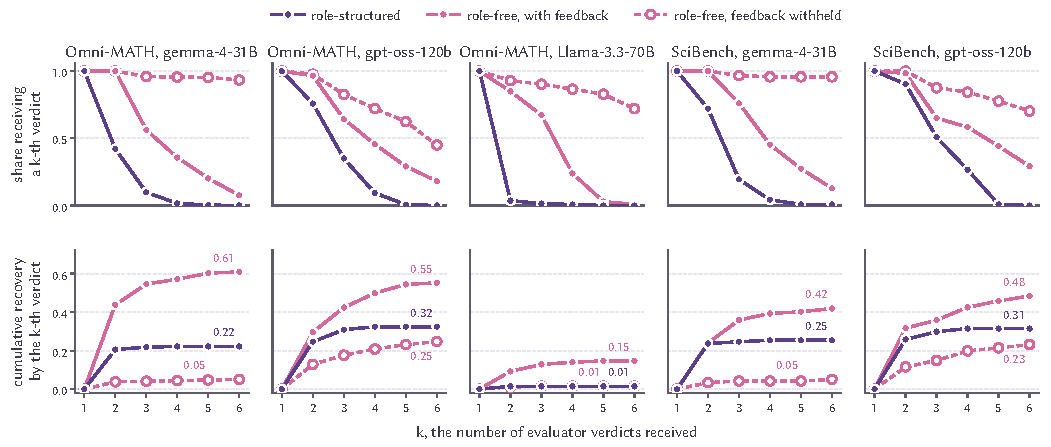
\includegraphics[width=\textwidth]{figures/fig_supp_verdicts.pdf}
\Description{Two rows of five panels, one column per cell. Top row: the
share of first-pass-wrong trajectories that receive a k-th verdict, falling
steeply for the role-structured team, more slowly for the role-free team
with feedback, and hardly at all for the role-free team without feedback.
Bottom row: cumulative recovery by the k-th verdict; the role-structured
curve flattens after the second verdict while the role-free curve with
feedback keeps rising.}
\caption{Recovery follows exposure to the evaluator. Top: the share of
first-pass-wrong trajectories that receive a $k$-th evaluator verdict.
Bottom: the cumulative share recovered by the $k$-th verdict, with the
final value labeled. One panel per cell (actor on benchmark):
role-structured (purple), role-free with feedback (rose) and role-free with
the feedback withheld (hollow, dashed). The role-structured curve flattens
where its trajectories stop receiving verdicts, not where they stop using
them.}
\label{fig:verdicts}
\end{figure*}

\paragraph{Recovery tracks exposure.} Figure~\ref{fig:verdicts} shows the
mechanism directly. In every cell the RS team's share of trajectories still
receiving verdicts falls steeply after the first one, while the RF team's
falls slowly, and the cumulative recovery curves follow the exposure
curves. Per verdict received, neither team is consistently ahead: on the paired
problems, pooled over the five cells, the share whose second verdict is a
PASS is $0.267$ for RS and $0.224$ for RF, and at the third and fourth
verdicts $0.083$ against $0.127$ and $0.105$ against $0.089$. Recoveries
per verdict after the first are higher with roles in every cell
(Table~\ref{tab:gate}), but that ratio compares different trajectories,
since most of the RF team's later verdicts are further attempts on problems
it has already failed more than once; the like-for-like comparison is the
verdict-matched one.

\paragraph{How far the verdict-matched comparison can be pushed.} Matching
on verdicts is coarse. When the RS team received a single verdict, because
it never submitted and was graded at the end or because it submitted once
and stopped, the RF trajectory cut to one verdict cannot recover either,
and the pair ties at zero by construction. These forced ties are most of
the gemma-4-31B-it pairs and nearly all of the Llama-3.3-70B-Instruct pairs
(Table~\ref{tab:robust}), so the pooled interval of the main text is
narrower than the information behind it. The cut is also one-sided, since
the RS count stops at that team's own passing verdict, which can only favor
it. Table~\ref{tab:robust} and Figure~\ref{fig:robustness}a therefore give
the contrast under six definitions: the problems with at least two RS
verdicts, both trajectories cut at the smaller count, and the scoring
defect recoded, each with and without Llama-3.3-70B-Instruct. No variant
puts the RF team significantly ahead: the two symmetric cuts favor it by
$0.005$ and $0.010$ with intervals that include zero, the informative
problems allow up to $+0.065$ in favor of roles ($+0.073$ with the
recoding), and with the recoding on all problems the RS team leads by
$+0.029$ with an interval that excludes zero. The defensible reading is the
main text's: matched on verdicts the RF advantage disappears, and any
per-verdict advantage of roles is small. Matching equalizes exposure to the
evaluator, not calls; the RS team spends more cycles per verdict.

% Workshop copy (scripts/mk_workshop_appendix.py): paper/tables/verdict_robustness.tex with its tabular in an adjustbox; numbers unchanged.
%% GENERATED by analysis/scripts/mk_robust_table.py from FIGDATA_GATE.json
%% (bf_gate.py [G4], [G6]) -- do not edit by hand.
\begin{table*}[t]
\centering
\caption{Robustness of the verdict-matched recovery contrast: forced ties, six definitions of the contrast, and per-verdict pass rates.}
\label{tab:robust}
\begin{adjustbox}{max width=\textwidth}\begin{tabular}{@{}l ccccc@{}}
\toprule
cell & paired $n$ & forced ties & RS never submitted & problems left & held-answer recodes (RS / RF) \\
\midrule
gemma-4-31B-it, Omni-MATH & $236$ & $141$ & $66$ & $95$ & $12$ / $3$ \\
gpt-oss-120b, Omni-MATH & $319$ & $84$ & $36$ & $235$ & $4$ / $0$ \\
Llama-3.3-70B-Instruct, Omni-MATH & $250$ & $242$ & $187$ & $8$ & $2$ / $1$ \\
gemma-4-31B-it, SciBench & $100$ & $29$ & $2$ & $71$ & $2$ / $0$ \\
gpt-oss-120b, SciBench & $93$ & $11$ & $1$ & $82$ & $0$ / $0$ \\
\bottomrule
\end{tabular}\end{adjustbox}

\vspace{4pt}
\begin{adjustbox}{max width=\textwidth}\begin{tabular}{@{}l c l c c l@{}}
\toprule
 & \multicolumn{3}{c}{all five cells} & \multicolumn{2}{c}{without Llama-3.3} \\
\cmidrule(lr){2-4}\cmidrule(lr){5-6}
definition & $n$ & difference [95\% interval] & equivalent & $n$ & difference [95\% interval] \\
\midrule
all paired problems (as in the main text's Table~2) & $998$ & $+0.009$ {\footnotesize $[{-}0.014,\,+0.033]$} & yes & $748$ & $+0.011$ {\footnotesize $[{-}0.020,\,+0.043]$} \\
problems with two or more role-structured verdicts & $491$ & $+0.018$ {\footnotesize $[{-}0.029,\,+0.065]$} & no & $483$ & $+0.017$ {\footnotesize $[{-}0.031,\,+0.064]$} \\
both cut at the smaller verdict count & $998$ & ${-}0.005$ {\footnotesize $[{-}0.029,\,+0.019]$} & yes & $748$ & ${-}0.008$ {\footnotesize $[{-}0.040,\,+0.024]$} \\
both cut, two or more verdicts & $491$ & ${-}0.010$ {\footnotesize $[{-}0.059,\,+0.039]$} & no & $483$ & ${-}0.012$ {\footnotesize $[{-}0.062,\,+0.037]$} \\
scoring defect recoded & $998$ & $+0.029$ {\footnotesize $[+0.004,\,+0.054]$} & no & $748$ & $+0.035$ {\footnotesize $[+0.003,\,+0.067]$} \\
recoded, two or more verdicts & $491$ & $+0.026$ {\footnotesize $[{-}0.020,\,+0.073]$} & no & $483$ & $+0.025$ {\footnotesize $[{-}0.023,\,+0.072]$} \\
\bottomrule
\end{tabular}\end{adjustbox}

\vspace{4pt}
\begin{adjustbox}{max width=\textwidth}\begin{tabular}{@{}l cc@{}}
\toprule
per-verdict pass rate & role-structured & role-free with feedback \\
\midrule
verdict 2 & $131/491=0.267$ & $212/946=0.224$ \\
verdict 3 & $19/228=0.083$ & $89/700=0.127$ \\
verdict 4 & $8/76=0.105$ & $39/439=0.089$ \\
\bottomrule
\end{tabular}\end{adjustbox}
\tabnote{RS: role-structured; RF: role-free with the evaluator's feedback shown; a cell is one actor on one benchmark. The contrast takes the problems both teams first answer wrongly and cuts the RF trajectory after as many evaluator verdicts as the RS trajectory received on that problem. Where RS received a single verdict, the cut RF trajectory cannot recover either, so the pair ties at zero by construction. Upper block: such forced ties per cell, how many of them never submitted, the problems left, and the trajectories whose held answer matched the key but were graded wrong (the scoring defect of the main text's Limitations). Middle block: the pooled difference, RS minus RF, stratified by cell with 95\% bootstrap intervals over problems, under six definitions, with and without Llama-3.3-70B-Instruct; equivalent means the 90\% interval lies inside $\pm0.05$. Recoding counts an RS trajectory with a correct held answer as recovered, and an RF one only if it was not cut. Lower block: the share of trajectories whose $k$-th verdict is PASS among those whose earlier verdicts all failed, pooled over the five cells.}
\end{table*}


\begin{figure*}[t]
\centering
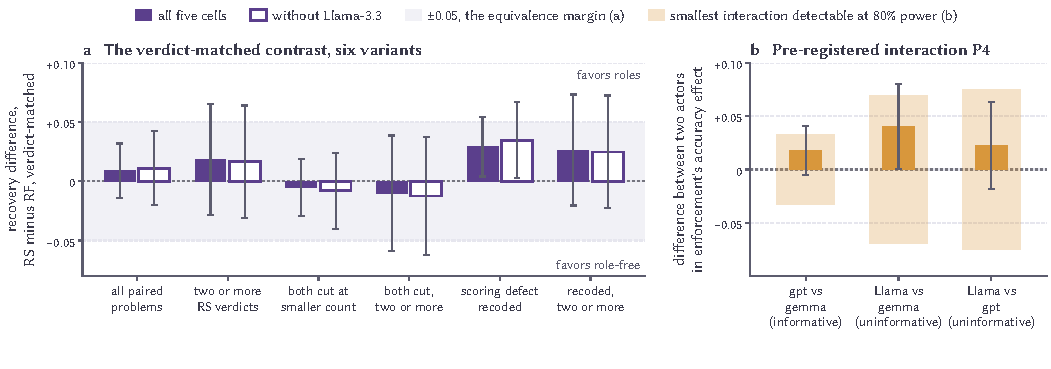
\includegraphics[width=\textwidth]{figures/fig_supp_robustness.pdf}
\Description{Two bar charts with error bars. Left: six pairs of bars,
one pair per definition of the verdict-matched contrast, all small and
with intervals that cross or nearly cross zero, inside a shaded band from
minus 0.05 to plus 0.05. Right: three bars for the pre-registered
interaction, each with an interval, drawn over a wider shaded bar showing
the smallest detectable effect; for two of the three the shaded bar is
wider than the band.}
\caption{Two robustness checks. (a) The verdict-matched recovery
difference, role-structured minus role-free with feedback, pooled over the
five cells (filled) and without Llama-3.3-70B-Instruct (hollow), under the
six definitions of Table~\ref{tab:robust}, with $95\%$ intervals; the band
marks the $\pm0.05$ equivalence margin. (b) The pre-registered interaction
P4 (Appendix~\ref{sec:prereg}): each difference between two actors in
enforcement's effect on final accuracy, with its $95\%$ interval; the
shaded bar behind it spans the smallest interaction detectable at $80\%$
power. Where that bar is wider than any plausible effect, the null is
uninformative.}
\label{fig:robustness}
\end{figure*}

\paragraph{Across the freeze.} The frozen RS cell and the RF team were run
on opposite sides of the freeze, so we repeat the comparison against the
post-freeze RS re-run of gemma-4-31B-it on $400$ Omni-MATH problems. On the
$65$ problems both first answer wrongly, the RF team leads $22$ to $3$
unmatched ($p=1.6\times10^{-4}$), but the RS team leads $4$ to $1$
verdict-matched ($p=0.38$): the same pattern as in the frozen comparison.

\paragraph{Removing the gate alone.} The forced-submission run tests the
gate directly. It uses the RS prompts and runner unchanged except for one
step: after the Reviewer's turn, the pipeline submits the team's current
answer to the evaluator whatever route the Reviewer chose, and the verdict
and hint reach the agents through the same role-specific slots as in the RS
condition. An offline test (no model calls), to be released with the code,
checks that the prompts are byte-identical to the RS ones up to the first
verdict and that the evaluator is called in every cycle. It was run once,
after the freeze, for gemma-4-31B-it on the $400$ Omni-MATH problems of the
RS re-run, with the same server, budget and evaluator.
Table~\ref{tab:forced} compares it with that re-run, the frozen RS cell and
the RF team, restricted to the same problems. Recovery rises to the RF
team's level while first-pass accuracy does not move: once the Reviewer's
approvals no longer decide anything, the role prompts recover as much as
the generic ones.

% Workshop copy (scripts/mk_workshop_appendix.py): paper/tables/forced_submission.tex with its tabular in an adjustbox; numbers unchanged.
%% GENERATED by analysis/scripts/mk_afs_table.py from FIGDATA_GATE.json
%% (bf_gate.py [G5]) -- do not edit by hand.
\begin{table*}[t]
\centering
\caption{Removing the submission gate: gemma-4-31B-it on the same $400$ Omni-MATH problems in every row.}
\label{tab:forced}
\begin{adjustbox}{max width=\textwidth}\begin{tabular}{@{}l ccccc@{}}
\toprule
condition & first pass & recovery & final accuracy & verdicts & Reviewer approvals \\
\midrule
role-structured, every cycle submitted & $0.768$ & $57/93=0.613$ & $0.910$ & $4.20$ & $0.98$ \\
role-structured, re-run after the freeze & $0.773$ & $18/91=0.198$ & $0.818$ & $1.44$ & $1.13$ \\
role-structured, frozen snapshot & $0.795$ & $12/82=0.146$ & $0.825$ & $1.41$ & $1.15$ \\
role-free with feedback & $0.795$ & $45/82=0.549$ & $0.908$ & $3.34$ & $3.34$ \\
\bottomrule
\end{tabular}\end{adjustbox}

\vspace{4pt}
\begin{adjustbox}{max width=\textwidth}\begin{tabular}{@{}l ccc cc@{}}
\toprule
 & \multicolumn{3}{c}{recovery (both first wrong)} & \multicolumn{2}{c}{final accuracy} \\
\cmidrule(lr){2-4}\cmidrule(lr){5-6}
pair & $n$ & first / second only & $p$ & first / second only & $p$ \\
\midrule
every cycle submitted vs.\ re-run & $72$ & $26$ / $2$ & $3.0{\times}10^{-6}$ & $42$ / $5$ & $2.5{\times}10^{-8}$ \\
every cycle submitted vs.\ role-free with feedback & $70$ & $7$ / $7$ & $1$ & $8$ / $7$ & $1$ \\
re-run vs.\ role-free with feedback & $65$ & $3$ / $22$ & $1.6{\times}10^{-4}$ & $6$ / $42$ & $1.0{\times}10^{-7}$ \\
\bottomrule
\end{tabular}\end{adjustbox}
\tabnote{Role-structured: Planner, Executor and Reviewer prompts, in the frozen snapshot and in a re-run after the freeze; role-free with feedback: one generic prompt for all three agents, with the evaluator's feedback shown. The forced-submission run (``every cycle submitted'') uses the role-structured prompts byte for byte, but the pipeline submits the team's answer in every cycle whatever the Reviewer decides; its approvals are logged but do not decide submission. First pass: the share of trajectories whose first submitted answer is correct. Recovery: first-pass-wrong trajectories that finish correct, over each row's own first-pass-wrong set (count / denominator). Final accuracy: over all problems, never-graded trajectories counted as incorrect. Verdicts and Reviewer approvals: per first-pass-wrong trajectory, including the first. The lower block pairs two conditions on the problems both first answer wrongly (recovery) and on all problems (final accuracy): problems solved only by the first / only by the second, with the exact McNemar $p$ for the two counts.}
\end{table*}


\section{The second domain (R4)}
\label{sec:xdomain}

Table~\ref{tab:scibench} gives the SciBench feedback-withheld comparison
in full: the frozen RS and RF$^{-}$ cells with their denominators, for the
two actors run there. The main comparison, with feedback, is in the main text's Figure~2 and Table~2.

% Workshop copy (scripts/mk_workshop_appendix.py): paper/tables/scibench_replication.tex with its tabular in an adjustbox; numbers unchanged.
% ==========================================================================
% Table 3 (manuscript) -- SciBench cross-domain replication
%
% GENERATED FILE -- do not edit by hand. Any edit is overwritten.
% generating script : analysis/scripts/mk_tables.py
% canonical input   : analysis/scripts/xdom_analyze.py (executed; stdout parsed)
%                      which execs FINAL_TABLES.py and rebinds its definitions
%                      -- judged / is_fpw / fp / fin_prereg are the SAME code
%                      objects as the Omni-MATH tables, not a reimplementation
% frozen data       : experiments/results/FROZEN/, frozen_at 2026-09-30T10:09:30.201557
%                     11600 trajectories
%                     sha256 fa22a446d5314bb67b1c6a6444b511eeeae3eb8770419a36f182617eeccbf3b5  actor3.jsonl
%                     sha256 038e08aec4d4aee166106a6325309dfe2301faf339c7d0bf82338a74576424d4  armCp.jsonl
%                     sha256 e4e53cb117d91129991ce2fe87e336e152fc9ee6ca826d363f2bd5dd240d7130  campaign_v2.jsonl
% canonical-output sha256 : b26ccb5451a5eaed14046a27a980ba8797e5669912df907bc25f69bf60ad5b76
% generation date   : 2026-10-04  (derived from the canonical
%                     input's mtime, not wall-clock: regeneration must
%                     be byte-identical)
%
% SciBench frozen data: experiments/results/xdomain/FROZEN_SCIBENCH/
%   frozen_at 2026-09-30T23:26:47.198588+00:00, 2296 trajectories
%   sha256 10068f72cfd936d3be6de85fef196d63fc154ef2c2ec26a0ac2c7313513dce58  scibench_AB.jsonl
% gpt-oss's recovery cell is UNDERPOWERED:
% its point estimate matches Omni-MATH's. Llama-3.3 was not run.
% No clause-specific role-fidelity metric crosses domains (the
% contract was domain-adapted), so none is reported here.
%
% Reader-facing condition names per paper/TERMINOLOGY.md; internal arm
% codes are deliberately absent and their absence is asserted at
% generation time.
% ==========================================================================
\begin{table*}[t]
\centering
\caption{The SciBench benchmark: first pass and recovery with roles and without them (feedback withheld), two actors, frozen separately.}
\label{tab:scibench}
\begin{adjustbox}{max width=\textwidth}\begin{tabular}{lccccc@{\hspace{1.4em}}ccccccc}
\toprule
 & \multicolumn{5}{c}{first pass (paired, all problems)}
 & \multicolumn{7}{c}{recovery (paired on first-pass wrong under both)} \\
\cmidrule(lr){2-6}\cmidrule(lr){7-13}
actor & $n$ & RS & RF$^{-}$ & diff. & exact $p$
      & $n_{\mathrm{both}}$ & RS & RF$^{-}$ & diff.
      & RS only & RF$^{-}$ only & exact $p$ \\
\midrule
gemma-4-31B-it & $574$ & $0.794$ & $0.794$ & $+0.0000$ & $1$ & $99$ & $0.212$ & $0.020$ & ${-}0.1919$ & $21$ & $2$ & $6.60\times 10^{-5}$ \\
gpt-oss-120b & $574$ & $0.784$ & $0.789$ & $+0.0052$ & $0.784$ & $96$ & $0.219$ & $0.135$ & ${-}0.0833$ & $17$ & $9$ & $0.169$ \\
\bottomrule
\end{tabular}\end{adjustbox}
\tabnote{The complete 574-problem text-only slice of free-response college science, 2,296 trajectories. RS: role-structured; RF$^{-}$: role-free with the evaluator's feedback withheld; the contrast with feedback shown is in the main text's Table~2. First pass is paired over all 574 problems, with the exact McNemar $p$ for the problems right under only one condition. Recovery is paired over only the problems first-pass wrong under both conditions ($n_{\mathrm{both}}$); ``RS only'' and ``RF$^{-}$ only'' count problems recovered under one condition and not the other. Differences are RF$^{-}$ minus RS under the pre-registered scoring (never-graded trajectories count as incorrect). gpt-oss-120b's recovery cell is underpowered at its $n_{\mathrm{both}}$; its estimate points the same way as on Omni-MATH. Llama-3.3-70B-Instruct was not run in this domain.}
\end{table*}


\paragraph{What was and was not changed.} The prompts are not byte-identical
to Omni-MATH's, and the prompt files, to be released with the code, make the
difference checkable. Of the $16$ prompts the two domains share, $11$ are
identical and $5$ differ: four of the six RS prompts (the Planner, Executor
and Reviewer preambles and the Reviewer's routing rules) and the evaluator's
preamble, which must ask for scientific rather than mathematical
equivalence. Both RF prompts are identical across domains, as are the six SE
prompts (enforcement was not run on SciBench). The asymmetry deserves
stating plainly: the RS prompts, whose team recovers less than the RF team,
are the ones that were rewritten, while the RF prompts ran identical text in
both domains. The rewrite is domain wording (``algebraic manipulation or
numerical calculation'' where Omni-MATH said ``symbolic manipulation or
arithmetic''), and the structural clauses are unchanged; a reader who
suspects the adaptation is doing the work can check the files once they are released. Topology,
budget, decoding, retry policy and the evaluator protocol are unchanged, so
this is a replication of the mechanism under a matched protocol, not a
rerun of identical prompts.

\paragraph{Why the answer does not lock here.} On Omni-MATH the
gemma-4-31B-it RS team often keeps the same answer across cycles (a single
distinct answer in $28.8\%$ of its failed trajectories); on SciBench it does
not ($7.6\%$, against $8.5\%$ for the RF team). The RS team on SciBench also
almost always submits at least once (Table~\ref{tab:gate}), so it sees more
feedback, and by the second verdict the two teams have recovered equally often. A looser
gate is the simplest common explanation of both observations, though we did
not test it.

\section{Structural enforcement (R4)}
\label{sec:enforcement}

The main text reports that enforcement loosens the gate and raises
recovery, but that attrition keeps the gain from reaching end-to-end
accuracy, and that the apparent accuracy benefit under the as-graded scoring
is survivorship. Table~\ref{tab:enforcement} and
Figure~\ref{fig:enforcement} are the evidence for both halves: the
manipulation check, the one-sided attrition, and the same accuracy
difference under both scorings.

% Workshop copy (scripts/mk_workshop_appendix.py): paper/tables/structural_enforcement.tex with its tabular in an adjustbox; numbers unchanged.
% ==========================================================================
% Table 4 (manuscript) -- structural enforcement
%
% GENERATED FILE -- do not edit by hand. Any edit is overwritten.
% generating script : analysis/scripts/mk_tables.py
% canonical input   : analysis/out/FINAL_TABLES_OUTPUT.txt  sections T1, T2, T7, T11
% frozen data       : experiments/results/FROZEN/, frozen_at 2026-09-30T10:09:30.201557
%                     11600 trajectories
%                     sha256 fa22a446d5314bb67b1c6a6444b511eeeae3eb8770419a36f182617eeccbf3b5  actor3.jsonl
%                     sha256 038e08aec4d4aee166106a6325309dfe2301faf339c7d0bf82338a74576424d4  armCp.jsonl
%                     sha256 e4e53cb117d91129991ce2fe87e336e152fc9ee6ca826d363f2bd5dd240d7130  campaign_v2.jsonl
% canonical-output sha256 : b26ccb5451a5eaed14046a27a980ba8797e5669912df907bc25f69bf60ad5b76
% generation date   : 2026-10-04  (derived from the canonical
%                     input's mtime, not wall-clock: regeneration must
%                     be byte-identical)
%
% The manipulation-check column is ANSWER AUTHORSHIP = 1 minus
% T11's 'authored-free' column, which is a FREEDOM rate. The
% manuscript once read that axis inverted (APPROVED_CLAIMS A11);
% the complement is taken here, once, in code.
% Recovery denominator as in Table 2 (judged & fp==0).
% APPROVED_CLAIMS A6: enforcement restores recovery for Llama-3.3
% ONLY. For the other two the direction is consistent but not
% resolvable. 'Highest of any arm, above role-structured in all
% three actors' is a DEAD claim and must not reappear.
% The as-graded column is SENSITIVITY ONLY -- it is the
% survivorship reading, which is why attrition sits beside it.
%
% Reader-facing condition names per paper/TERMINOLOGY.md; internal arm
% codes are deliberately absent and their absence is asserted at
% generation time.
% ==========================================================================
\begin{table*}[t]
\centering
\caption{Structural enforcement against the role-structured baseline on the Omni-MATH benchmark: the manipulation check, attrition, and final accuracy under both scorings.}
\label{tab:enforcement}
\begin{adjustbox}{max width=\textwidth}\begin{tabular}{lccccccc}
\toprule
 & Planner authors & locked answer & recovery & &
 \multicolumn{2}{c}{final accuracy, SE $-$ RS} \\
\cmidrule(lr){6-7}
actor & answer (RF$^{-}$) & (RF$^{-}$ / RS) & (RS) & attrition
      & pre-registered & as graded \\
\midrule
gemma-4-31B-it & $0.000$ (0.986) & $0.119$ (0.845/0.288) & $0.314$ (0.222) & $8.0\%$ & ${-}0.0225$ {\footnotesize [-0.0387,-0.0063]} & $+0.0190$ {\footnotesize [+0.0054,+0.0333]} \\
gpt-oss-120b & $0.000$ (0.916) & $0.092$ (0.208/0.052) & $0.395$ (0.324) & $9.9\%$ & ${-}0.0050$ {\footnotesize [-0.0219,+0.0112]} & $+0.0361$ {\footnotesize [+0.0215,+0.0507]} \\
Llama-3.3-70B-Instruct & $0.000$ (0.958) & $0.072$ (0.806/0.750) & $0.139$ (0.014) & $17.0\%$ & $+0.0175$ {\footnotesize [-0.0200,+0.0550]} & $+0.0453$ {\footnotesize [+0.0030,+0.0876]} \\
\bottomrule
\end{tabular}\end{adjustbox}

\tabnote{SE: structurally enforced; RS: role-structured; RF$^{-}$: role-free with the evaluator's feedback withheld. Planner authors answer: the share of Planner messages that state a final answer, under SE and (in parentheses) under RF$^{-}$; SE drives it to zero in all three actors, so the intervention engaged (the manipulation check). Locked answer: the share of first-pass-wrong trajectories whose answer string never changed, under SE and (in parentheses) RF$^{-}$ / RS. Recovery: the share of first-pass-wrong trajectories that finish correct, under SE and (in parentheses) RS, on the denominator of Table~\ref{tab:recovery}. Attrition: the share of SE trajectories that never finish because a malformed output exhausted its regeneration budget. Final accuracy: the difference over all problems with 95\% bootstrap intervals, under the pre-registered scoring (never-graded trajectories count as incorrect) and as graded (they are dropped); the two columns are different populations and the attrition column is why they disagree. Attrition elsewhere is negligible: $0.0$--$0.8\%$ with roles,
$0.0$--$2.5\%$ without. The as-graded column turns every sign
positive; the pre-registration fixed in advance that unparseable
trajectories count incorrect, and \textbf{the benefit appears only after
conditioning on successful parsing.}}
\end{table*}


\begin{figure}[t]
\centering
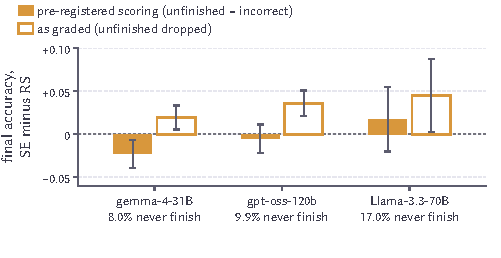
\includegraphics[width=0.585\textwidth]{figures/fig_supp_enforcement.pdf}
\Description{A bar chart with error bars. For each of three actors, two
bars of the accuracy difference between the enforced and the
role-structured condition, one under the pre-registered scoring and one as
graded; the as-graded bar is higher than the pre-registered one in every
group. The tick labels give each actor's share of enforced trajectories
that never finish, from 8 percent to 17 percent.}
\caption{Enforcement's effect on final accuracy under the two scorings.
Enforced minus role-structured final accuracy per actor with $95\%$
intervals, under the pre-registered scoring (unfinished trajectories count
as incorrect; filled) and as graded (they are dropped; hollow). The tick
labels give the share of enforced trajectories that never finish, which is
what separates the two bars. The sign flips between the scorings for two
of the three actors, and the as-graded gains are ordered like the
attrition.}
\label{fig:enforcement}
\end{figure}

\paragraph{Why the columns do not compose.} The enforced recovery and
first-pass rates do not combine into the accuracy column, and cannot:
trajectories that never receive a first verdict have no first pass, and
those that die after one stay in the recovery denominator, so the three
quantities do not share a denominator. The pre-registration fixed in advance
that unparseable trajectories count as incorrect rather than being dropped,
and that rule is what makes the as-graded reading survivorship rather than a
finding.

\paragraph{The gate loosens, and brittleness follows the same order.} Per
failed trajectory, the SE Reviewer approves $2.02$, $2.33$ and $1.84$ times
for gemma-4-31B-it, gpt-oss-120b and Llama-3.3-70B-Instruct, against
$1.27$, $2.10$ and $0.32$ under RS prompts. Enforcement logs $838$,
$1{,}183$ and $395$ role-boundary rejections, that is $0.52$, $0.74$ and
$0.99$ per trajectory, in the same order as the attrition ($8.0\%$, $9.9\%$
and $17.0\%$): the actor that breaks the schema most often is the one that
loses the most trajectories. For Llama-3.3-70B-Instruct, whose RS team
rarely submits, enforced recovery comes close to the RF team's ($0.139$
against $0.147$); on the $219$ problems both first answer wrongly, $9$ are
recovered only under enforcement and $17$ only by the RF team ($p=0.17$).

\paragraph{The context-restored control.} Enforcement also hides the
shared history from the Executor, so part of its brittleness may be lost
context rather than the typed interface. Restoring the shared history
at fixed enforcement (gemma-4-31B-it and gpt-oss-120b, $400$ problems each;
attrition $4.5\%$ and $9.8\%$) changes final accuracy relative to
enforcement by $+0.0450$ $[+0.0125,+0.0775]$ ($p=0.0079$) for gemma-4-31B-it
and by $-0.0125$ $[-0.0475,+0.0200]$ ($p=0.56$) for gpt-oss-120b under the
pre-registered scoring, and by $+0.0196$ $[-0.0028,+0.0419]$ ($p=0.14$) and
$-0.0089$ $[-0.0357,+0.0149]$ ($p=0.65$) as graded. For gemma-4-31B-it the
gain is significant only under the scoring that penalizes attrition, so it
comes mostly from fewer trajectories dying; the control is partial, because
the attrition it removes is one-sided.

% Workshop copy (scripts/mk_workshop_appendix.py): paper/tables/prereg_endpoints.tex with its tabular in an adjustbox; numbers unchanged.
% ==========================================================================
% Table 6 (supplement) -- pre-registered endpoints
%
% GENERATED FILE -- do not edit by hand. Any edit is overwritten.
% generating script : analysis/scripts/mk_tables.py
% canonical input   : analysis/out/FINAL_TABLES_OUTPUT.txt  sections T2, T14, T29
%                    analysis/scripts/stat_audit_a7_power.py (executed) -- MDE only
% frozen data       : experiments/results/FROZEN/, frozen_at 2026-09-30T10:09:30.201557
%                     11600 trajectories
%                     sha256 fa22a446d5314bb67b1c6a6444b511eeeae3eb8770419a36f182617eeccbf3b5  actor3.jsonl
%                     sha256 038e08aec4d4aee166106a6325309dfe2301faf339c7d0bf82338a74576424d4  armCp.jsonl
%                     sha256 e4e53cb117d91129991ce2fe87e336e152fc9ee6ca826d363f2bd5dd240d7130  campaign_v2.jsonl
% canonical-output sha256 : b26ccb5451a5eaed14046a27a980ba8797e5669912df907bc25f69bf60ad5b76
% generation date   : 2026-10-04  (derived from the canonical
%                     input's mtime, not wall-clock: regeneration must
%                     be byte-identical)
%
% P4 -- THE pre-registered primary -- is NULL before and after
% Holm. Reported as the failure of the thesis it was written to
% test (APPROVED_CLAIMS A10).
% P1 FAILED AS WRITTEN and was re-designated: the schema forbids
% emitting an ANSWER, not performing COMPUTATION. Reported as a
% finding, not hidden (DECISION_LOG D9/R1).
% P2 and P5 yield no p-value and are not p-corrected; the Holm
% family is therefore P3's three contrasts and P4's three DiDs,
% which is what the canonical output corrects.
% 
% PREREG_MDE_POPULATION_NOTE -- the MDE column and the
% difference-in-difference column come from DIFFERENT
% populations and are not arithmetically consistent:
%   * T14's DiD differences two per-actor C-A means computed on
%     each actor's OWN problem set (n=1600 and n=400).
%   * the MDE is computed on problems shared by BOTH actors,
%     where the Llama/gemma-4 observed DiD is +0.0300, not the
%     +0.0400 T14 prints.
% Both are correct for their own question; the MDE is quoted only
% as a detectability scale, never as the effect estimate. Do not
% recompute one from the other.
%
% Reader-facing condition names per paper/TERMINOLOGY.md; internal arm
% codes are deliberately absent and their absence is asserted at
% generation time.
% ==========================================================================
\begin{table*}[t]
\centering
\caption{The five pre-registered endpoints and what each returned. P4, the primary, is null before and after Holm correction.}
\label{tab:prereg}
\begin{adjustbox}{max width=\textwidth}\begin{tabular}{@{}llllll@{}}
\toprule
endpoint & \multicolumn{5}{l}{disposition} \\
\midrule
\textbf{P1} intervention $\rightarrow$ fidelity
 & \multicolumn{5}{l}{\textbf{failed as written; re-designated.} The
   interface forbids an \emph{answer} field, not} \\
\quad \footnotesize(also the manipulation check)
 & \multicolumn{5}{l}{\quad computation. Re-scoped to answer authorship,
   which it drives to $0.000$ in all three} \\
 & \multicolumn{5}{l}{\quad actors (Table~\ref{tab:enforcement}).
   Reported as a second dissociation, not as a pass.} \\
\addlinespace
\textbf{P2} actor $\times$ interv.\ on fidelity
 & \multicolumn{5}{l}{not estimable across the panel: the fidelity
   clauses are condition-specific, so no} \\
 & \multicolumn{5}{l}{\quad common scale exists. Reported as unresolved
   rather than substituted.} \\
\addlinespace
\multicolumn{6}{@{}l}{\textbf{P3} intervention $\rightarrow$ accuracy
  (enforced $-$ role-structured), Holm across three:} \\
 & raw $p$ & Holm $p$ & verdict & & \\
\quad gemma-4-31B-it & $0.0078$ & $0.023$ & reject \\
\quad gpt-oss-120b & $0.60$ & $0.85$ & retain \\
\quad Llama-3.3-70B-Instruct & $0.43$ & $0.85$ & retain \\
\addlinespace
\multicolumn{6}{@{}l}{\textbf{P4} actor $\times$ intervention on
  accuracy (the pre-registered primary), Holm across three:} \\
 & difference-in-diff.\ [CI] & raw $p$ & Holm $p$ & MDE$_{80\%}$ & null is \\
\quad gpt-oss-120b $-$ gemma-4-31B-it & $+0.0175$ {\footnotesize [-0.0050,+0.0406]} & $0.145$ & $0.29$ & $0.0325$ & informative \\
\quad Llama-3.3-70B-Instruct $-$ gemma-4-31B-it & $+0.0400$ {\footnotesize [+0.0006,+0.0800]} & $0.0553$ & $0.166$ & $0.0693$ & uninformative \\
\quad Llama-3.3-70B-Instruct $-$ gpt-oss-120b & $+0.0225$ {\footnotesize [-0.0181,+0.0631]} & $0.286$ & $0.29$ & $0.0748$ & uninformative \\
\addlinespace
\textbf{P5} $\Delta$fidelity vs $\Delta$outcome
 & \multicolumn{5}{l}{association only, pre-declared as non-causal: both
   sides are outcomes of the same} \\
 & \multicolumn{5}{l}{\quad intervention. No $p$-value is reported and
   none is corrected.} \\
\bottomrule
\end{tabular}\end{adjustbox}

\tabnote{The endpoints were fixed in writing before any intervention data existed. The intervention is structural enforcement against the role-structured baseline, per actor. Fidelity: whether the Planner abstains from computing (\Pone{}). Accuracy: final accuracy over all problems, never-graded trajectories counted as incorrect. P3: exact McNemar test per actor, with the raw $p$, the $p$ after Holm's step-down correction across the three actors, and the verdict at $\alpha=0.05$. P4: each difference-in-differences is enforcement's effect in one actor minus its effect in another, with its 95\% bootstrap interval over problems, the raw and Holm-corrected $p$, and MDE$_{80\%}$, the smallest interaction detectable with 80\% power at the realized sample; a null is informative only where the MDE is below a plausible effect. P2 and P5 carry no $p$ value, so the testable contrasts are P3's three and P4's three; Holm across all six changes no verdict. P4's intervals and $p$ values come from two separately seeded bootstrap runs, so an interval can exclude zero while $p$ is just above 0.05; the MDE is computed on problems shared by both actors while each difference-in-differences uses each actor's own problems, so neither can be derived from the other. \textbf{Only one of the three P4 nulls is informative.} The
largest per-actor main effect is small enough that a true interaction is
plausibly ${\leq}0.040$; only the gpt-oss/gemma-4 contrast can see an
effect that size. The two Llama-3.3 contrasts cannot detect an interaction of
any plausible magnitude and are uninformative rather than evidence of
absence.}
\end{table*}

% Workshop copy (scripts/mk_workshop_appendix.py): paper/tables/context_quartiles.tex with its tabular in an adjustbox; numbers unchanged.
% ==========================================================================
% Supplement -- recovery by pooled context quartile
%
% GENERATED FILE -- do not edit by hand. Any edit is overwritten.
% generating script : analysis/scripts/mk_tables.py
% canonical input   : analysis/out/FINAL_TABLES_OUTPUT.txt  section T22
% frozen data       : experiments/results/FROZEN/, frozen_at 2026-09-30T10:09:30.201557
%                     11600 trajectories
%                     sha256 fa22a446d5314bb67b1c6a6444b511eeeae3eb8770419a36f182617eeccbf3b5  actor3.jsonl
%                     sha256 038e08aec4d4aee166106a6325309dfe2301faf339c7d0bf82338a74576424d4  armCp.jsonl
%                     sha256 e4e53cb117d91129991ce2fe87e336e152fc9ee6ca826d363f2bd5dd240d7130  campaign_v2.jsonl
% canonical-output sha256 : b26ccb5451a5eaed14046a27a980ba8797e5669912df907bc25f69bf60ad5b76
% generation date   : 2026-10-04  (derived from the canonical
%                     input's mtime, not wall-clock: regeneration must
%                     be byte-identical)
%
% DIRECTIONAL ONLY. Quartile cut points are POOLED over both
% conditions, and accumulated context is nearly a function of
% condition, so the strata are NOT balanced -- this cannot
% separate context from condition and must never be described
% as a controlled comparison or a mediation analysis.
% Cells with n<8 print '--' in the canonical output and stay
% suppressed here rather than being recomputed at low n.
%
% Reader-facing condition names per paper/TERMINOLOGY.md; internal arm
% codes are deliberately absent and their absence is asserted at
% generation time.
% ==========================================================================
\begin{table}[htb]
\centering
\caption{Recovery by accumulated-context quartile, with roles and without them (feedback withheld), on the Omni-MATH benchmark; directional only.}
\label{tab:context}
\begin{adjustbox}{max width=\textwidth}\begin{tabular}{@{}lccccc@{}}
\toprule
 & \multicolumn{2}{c}{RS} & \multicolumn{2}{c}{RF$^{-}$} & \\
\cmidrule(lr){2-3}\cmidrule(lr){4-5}
context quartile & recovery & $n$ & recovery & $n$ & difference \\
\midrule
\multicolumn{5}{@{}l}{\emph{gemma-4-31B-it}} \\
\quad Q1 (least context) & $0.662$ & $65$ & $0.151$ & $93$ & $+0.511$ \\
\quad Q2 & $0.280$ & $50$ & $0.009$ & $108$ & $+0.271$ \\
\quad Q3 & $0.047$ & $85$ & $0.014$ & $73$ & $+0.033$ \\
\quad Q4 (most) & $0.078$ & $116$ & $0.000$ & $42$ & $+0.078$ \\
\addlinespace
\multicolumn{5}{@{}l}{\emph{gpt-oss-120b}} \\
\quad Q1 (least context) & $0.923$ & $13$ & $0.258$ & $198$ & $+0.665$ \\
\quad Q2 & $0.656$ & $128$ & $0.293$ & $82$ & $+0.363$ \\
\quad Q3 & $0.262$ & $164$ & $0.191$ & $47$ & $+0.071$ \\
\quad Q4 (most) & $0.070$ & $158$ & $0.189$ & $53$ & ${-}0.119$ \\
\addlinespace
\multicolumn{5}{@{}l}{\emph{Llama-3.3-70B-Instruct}} \\
\quad Q1 (least context) & $0.100$ & $40$ & $0.031$ & $96$ & $+0.069$ \\
\quad Q2 & $0.000$ & $86$ & $0.000$ & $50$ & $+0.000$ \\
\quad Q3 & $0.000$ & $103$ & $0.030$ & $33$ & ${-}0.030$ \\
\quad Q4 (most) & $0.000$ & $47$ & $0.000$ & $89$ & $+0.000$ \\
\addlinespace
\bottomrule
\end{tabular}\end{adjustbox}
\tabnote{RS: role-structured; RF$^{-}$: role-free with the evaluator's feedback withheld. Recovery: the share of first-pass-wrong trajectories that finish correct, with $n$ the number of such trajectories in the quartile; the difference is RS minus RF$^{-}$. Context is the total character count of all agent messages in the trajectory; quartile cut points are computed once per actor over both conditions pooled. Because accumulated context is nearly a function of condition (the RF$^{-}$ team writes less because it stops changing its answer), the strata are not balanced and the comparison cannot separate context from condition.}
\end{table}

% Workshop copy (scripts/mk_workshop_appendix.py): paper/tables/single_agent_comparison.tex with its tabular in an adjustbox; numbers unchanged.
% ==========================================================================
% Table 5 (manuscript) -- budget-matched single-agent control
%
% GENERATED FILE -- do not edit by hand. Any edit is overwritten.
% generating script : analysis/scripts/mk_tables.py
% canonical input   : analysis/out/FINAL_TABLES_OUTPUT.txt  section T17
% frozen data       : experiments/results/FROZEN/, frozen_at 2026-09-30T10:09:30.201557
%                     11600 trajectories
%                     sha256 fa22a446d5314bb67b1c6a6444b511eeeae3eb8770419a36f182617eeccbf3b5  actor3.jsonl
%                     sha256 038e08aec4d4aee166106a6325309dfe2301faf339c7d0bf82338a74576424d4  armCp.jsonl
%                     sha256 e4e53cb117d91129991ce2fe87e336e152fc9ee6ca826d363f2bd5dd240d7130  campaign_v2.jsonl
% canonical-output sha256 : b26ccb5451a5eaed14046a27a980ba8797e5669912df907bc25f69bf60ad5b76
% generation date   : 2026-10-04  (derived from the canonical
%                     input's mtime, not wall-clock: regeneration must
%                     be byte-identical)
%
% PROVENANCE: NOT from the frozen snapshot. Source is the
% historical released trace corpus (protocol_id='single_agent',
% benchmark omnimath2), joined by problem_uid. This must be
% stated wherever the four numbers appear (APPROVED_CLAIMS A9).
% BOTH DIRECTIONS, ALWAYS TOGETHER. Never quote gpt-oss alone.
% The two actor arms were produced in SEPARATE RUNS:
% each direction is a sound guard; the GAP BETWEEN ACTORS is not.
%
% Reader-facing condition names per paper/TERMINOLOGY.md; internal arm
% codes are deliberately absent and their absence is asserted at
% generation time.
% ==========================================================================
\begin{table}[htb]
\centering
\caption{Each three-agent team against a single agent of the same actor under the same call cap, on the Omni-MATH benchmark.}
\label{tab:singleagent}
\begin{adjustbox}{max width=\textwidth}\begin{tabular}{@{}lccc@{}}
\toprule
organization & team & single agent & difference \\
\midrule
\multicolumn{4}{@{}l}{\emph{gemma-4-31B-it}} \\
\quad role-structured & $0.8462$ & $0.8688$ & ${-}0.0225$ \\
 & \multicolumn{3}{r}{\footnotesize $[{-}0.0400,\,{-}0.0056]$, $p=0.0122$, $n=1600$} \\
\quad role-free & $0.8125$ & $0.8688$ & ${-}0.0563$ \\
 & \multicolumn{3}{r}{\footnotesize $[{-}0.0737,\,{-}0.0394]$, $p=1.22\times 10^{-10}$, $n=1600$} \\
\addlinespace
\multicolumn{4}{@{}l}{\emph{gpt-oss-120b}} \\
\quad role-structured & $0.8031$ & $0.7900$ & $+0.0131$ \\
 & \multicolumn{3}{r}{\footnotesize $[{-}0.0044,\,+0.0300]$, $p=0.152$, $n=1600$} \\
\quad role-free & $0.8194$ & $0.7900$ & $+0.0294$ \\
 & \multicolumn{3}{r}{\footnotesize $[+0.0125,\,+0.0456]$, $p=0.000678$, $n=1600$} \\
\addlinespace
\midrule
\multicolumn{4}{@{}l}{\emph{Realized call budget}} \\
\midrule
actor & protocol & evaluator & actor \\
\midrule
gemma-4-31B-it & single agent & $1.66$ & $3.16$ \\
gemma-4-31B-it & role-structured team & $1.11$ & $6.76$ \\
gemma-4-31B-it & role-free team & $1.95$ & $5.87$ \\
gpt-oss-120b & single agent & $1.69$ & $3.40$ \\
gpt-oss-120b & role-structured team & $1.35$ & $7.54$ \\
gpt-oss-120b & role-free team & $1.85$ & $6.25$ \\
\bottomrule
\end{tabular}\end{adjustbox}
\tabnote{Final accuracy over all problems ($n$) of the role-structured (RS) and role-free, feedback-withheld (RF$^{-}$) teams against a single agent of the same actor solving the same problems under the same cap on model calls; the difference is team minus single agent, with its 95\% bootstrap interval over problems and the exact McNemar $p$. The single-agent trajectories come from an earlier, separately collected trace corpus, joined by problem, and its two actor arms were produced in separate runs: each direction within an actor is a sound guard, the gap between actors is not. Realized call budget: calls per problem to the evaluator and to the actor.}
\end{table}


\paragraph{An excluded early campaign.} The main run was gated on a smoke
test requiring non-zero boundary rejections with reasons logged,
answer-bearing calls equal across conditions, and a pinned backend. An early
campaign of $121$ trajectories, run at half the main run's token limit, is
excluded: in it, $74\%$ of enforcement rejections were outputs cut off at
the token limit mid-JSON rather than role-boundary violations. Truncation
was not condition-specific but its cost was, because a prose condition
tolerates a truncated message where the enforced one rejects unparseable
JSON, so pooling those rows would have produced a spurious ``enforcement
lowers accuracy'' result. They were never pooled.

\paragraph{Accumulated context as a competing explanation.} The RS team's
recovery advantage over the RF$^{-}$ team could in principle come from the
longer history it accumulates over its internal cycles rather than from the feedback
it sees. Table~\ref{tab:context} stratifies recovery by accumulated context.
The comparison is directional only: quartile cut points are computed over
both conditions pooled, and accumulated context is nearly a function of
condition, because the RF$^{-}$ team stops changing its answer, so the strata are not
balanced and context cannot be separated from condition. It is reported
because it does not behave uniformly. The gap survives in the lower
quartiles, but in gpt-oss-120b's top quartile the ordering reverses, as it
does on a handful of events in Llama-3.3-70B-Instruct's third, so more
context is not simply more recovery.


\section{The pre-registered endpoints in full}
\label{sec:prereg}

The main text reports that the pre-registered primary endpoint P4, whether
enforcement's effect on accuracy differs by actor, is null (\S\ref{subsec:prereg}), and Appendix~\ref{app:details} that the
\Pone{} manipulation objective failed. Table~\ref{tab:prereg} is the
complete endpoint table: all five endpoints as written before any
intervention data existed, what each one returned, and the Holm-corrected
verdict.

Two things in it should be read rather than skimmed. First, only one of the
three P4 contrasts is an informative null (Figure~\ref{fig:robustness}b):
the largest per-actor main effect is small enough that a true interaction
is plausibly at most $0.040$, only the gpt-oss-120b against gemma-4-31B-it
contrast can detect an effect of that size, and the two contrasts involving
Llama-3.3-70B-Instruct cannot detect an interaction of any plausible
magnitude at their sample size. They are uninformative rather than evidence
of absence. Second, the contrast pre-registered as secondary and exploratory was RS
against RF$^{-}$; the contrast this paper is organized around, RS against
RF, and the forced-submission run are outside the pre-registration; the RF
condition's design and primary analysis were committed in writing before
its data existed, but its results are exploratory, and the main text
labels them so.

\section{The single-agent comparator}
\label{sec:singleagent}

Table~\ref{tab:singleagent} is the single-agent reference under the same
call cap. The main text uses it as a guard against reading ``collapse costs
nothing'' as ``the system was one agent all along'', and reports both
directions. The result cuts both ways: a collapsed gpt-oss-120b team beats
its own single agent, so three agents emitting one answer are not
functionally one agent, while gemma-4-31B-it's team is significantly worse
than its own single agent in both conditions. Neither ``multi-agent systems
are just single agents'' nor ``more agents help'' survives it. The
comparator comes from an earlier, separately collected corpus whose two
actor arms were produced in separate runs, so each direction within an
actor is a sound guard and the gap between actors is not.

\section{AI use statement}

In this work, we used generative AI tools for three purposes: to edit the
manuscript for readability and polish its wording; to search for and identify
relevant literature and to format references; and to assist with data
processing and analysis, including drafting and refining the code for these
tasks and for the figures. All AI-generated text and code were reviewed by the
authors, and LLM-generated code was verified and tested for correctness by the
authors. We take responsibility for the final content of this work, including
text, claims or artifacts produced with the aid of generative AI.


\end{document}
